\documentclass[a4paper]{book}
\usepackage{makeidx}
\usepackage{graphicx}
\usepackage{multicol}
\usepackage{float}
\usepackage{listings}
\usepackage{color}
\usepackage{ifthen}
\usepackage[table]{xcolor}
\usepackage{textcomp}
\usepackage{alltt}
\usepackage{ifpdf}
\ifpdf
\usepackage[pdftex,
            pagebackref=true,
            colorlinks=true,
            linkcolor=blue,
            unicode
           ]{hyperref}
\else
\usepackage[ps2pdf,
            pagebackref=true,
            colorlinks=true,
            linkcolor=blue,
            unicode
           ]{hyperref}
\usepackage{pspicture}
\fi
\usepackage[utf8]{inputenc}
\usepackage{mathptmx}
\usepackage[scaled=.90]{helvet}
\usepackage{courier}
\usepackage{doxygen}
\lstset{language=C++,inputencoding=utf8,basicstyle=\footnotesize,breaklines=true,breakatwhitespace=true,tabsize=8,numbers=left }
\makeindex
\setcounter{tocdepth}{3}
\renewcommand{\footrulewidth}{0.4pt}
\begin{document}
\hypersetup{pageanchor=false}
\begin{titlepage}
\vspace*{7cm}
\begin{center}
{\Large SimuladorDeSupermercado \\[1ex]\large ProjetoDeImplementacao1 }\\
\vspace*{1cm}
{\large Generated by Doxygen 1.7.3}\\
\vspace*{0.5cm}
{\small Thu Nov 15 2012 21:18:32}\\
\end{center}
\end{titlepage}
\clearemptydoublepage
\pagenumbering{roman}
\tableofcontents
\clearemptydoublepage
\pagenumbering{arabic}
\hypersetup{pageanchor=true}
\chapter{Namespace Index}
\section{Namespace List}
Here is a list of all namespaces with brief descriptions:\begin{DoxyCompactList}
\item\contentsline{section}{\hyperlink{namespaceProjeto1}{Projeto1} }{\pageref{namespaceProjeto1}}{}
\end{DoxyCompactList}

\chapter{Class Index}
\section{Class Hierarchy}
This inheritance list is sorted roughly, but not completely, alphabetically:\begin{DoxyCompactList}
\item \contentsline{section}{Projeto1::Caixa}{\pageref{classProjeto1_1_1Caixa}}{}
\begin{DoxyCompactList}
\item \contentsline{section}{Projeto1::CaixaEspecial}{\pageref{classProjeto1_1_1CaixaEspecial}}{}
\end{DoxyCompactList}
\item \contentsline{section}{Projeto1::Cliente}{\pageref{classProjeto1_1_1Cliente}}{}
\item \contentsline{section}{Projeto1::ElementoDeFila}{\pageref{classProjeto1_1_1ElementoDeFila}}{}
\item \contentsline{section}{Projeto1::ElementoDeListaCircular}{\pageref{classProjeto1_1_1ElementoDeListaCircular}}{}
\item \contentsline{section}{Projeto1::ListaCircular}{\pageref{classProjeto1_1_1ListaCircular}}{}
\item \contentsline{section}{Projeto1::Supermercado}{\pageref{classProjeto1_1_1Supermercado}}{}
\end{DoxyCompactList}

\chapter{Class Index}
\section{Class List}
Here are the classes, structs, unions and interfaces with brief descriptions:\begin{DoxyCompactList}
\item\contentsline{section}{\hyperlink{classProjeto1_1_1Caixa}{Projeto1::Caixa} }{\pageref{classProjeto1_1_1Caixa}}{}
\item\contentsline{section}{\hyperlink{classProjeto1_1_1CaixaEspecial}{Projeto1::CaixaEspecial} }{\pageref{classProjeto1_1_1CaixaEspecial}}{}
\item\contentsline{section}{\hyperlink{classProjeto1_1_1Cliente}{Projeto1::Cliente} }{\pageref{classProjeto1_1_1Cliente}}{}
\item\contentsline{section}{\hyperlink{classProjeto1_1_1ElementoDeFila}{Projeto1::ElementoDeFila} }{\pageref{classProjeto1_1_1ElementoDeFila}}{}
\item\contentsline{section}{\hyperlink{classProjeto1_1_1ElementoDeListaCircular}{Projeto1::ElementoDeListaCircular} }{\pageref{classProjeto1_1_1ElementoDeListaCircular}}{}
\item\contentsline{section}{\hyperlink{classProjeto1_1_1ListaCircular}{Projeto1::ListaCircular} }{\pageref{classProjeto1_1_1ListaCircular}}{}
\item\contentsline{section}{\hyperlink{classProjeto1_1_1Supermercado}{Projeto1::Supermercado} }{\pageref{classProjeto1_1_1Supermercado}}{}
\end{DoxyCompactList}

\chapter{File Index}
\section{File List}
Here is a list of all files with brief descriptions:\begin{DoxyCompactList}
\item\contentsline{section}{src/\hyperlink{HeapSort_8cpp}{HeapSort.cpp} }{\pageref{HeapSort_8cpp}}{}
\item\contentsline{section}{src/\hyperlink{HeapSort_8h}{HeapSort.h} }{\pageref{HeapSort_8h}}{}
\item\contentsline{section}{src/\hyperlink{Main_8cpp}{Main.cpp} }{\pageref{Main_8cpp}}{}
\end{DoxyCompactList}

\chapter{Namespace Documentation}
\hypertarget{namespaceProjeto1}{
\section{Projeto1 Namespace Reference}
\label{namespaceProjeto1}\index{Projeto1@{Projeto1}}
}
\subsection*{Classes}
\begin{DoxyCompactItemize}
\item 
class \hyperlink{classProjeto1_1_1Caixa}{Caixa}
\item 
class \hyperlink{classProjeto1_1_1CaixaEspecial}{CaixaEspecial}
\item 
class \hyperlink{classProjeto1_1_1Cliente}{Cliente}
\item 
class \hyperlink{classProjeto1_1_1ElementoDeListaCircular}{ElementoDeListaCircular}
\item 
class \hyperlink{classProjeto1_1_1ElementoDeFila}{ElementoDeFila}
\item 
class \hyperlink{classProjeto1_1_1ListaCircular}{ListaCircular}
\item 
class \hyperlink{classProjeto1_1_1Supermercado}{Supermercado}
\end{DoxyCompactItemize}
\subsection*{Enumerations}
\begin{DoxyCompactItemize}
\item 
enum \hyperlink{namespaceProjeto1_a4dade362b39c779d6411abf4ba19aeed}{TipoCliente} \{ \hyperlink{namespaceProjeto1_a4dade362b39c779d6411abf4ba19aeeda3c2a34a5670e3315f0c5493a00890611}{BuscaMenorFila}, 
\hyperlink{namespaceProjeto1_a4dade362b39c779d6411abf4ba19aeedaec1ed9ba7657b9ea20b55bada08f1825}{BuscaFilaComMenosProdutos}
 \}
\end{DoxyCompactItemize}


\subsection{Enumeration Type Documentation}
\hypertarget{namespaceProjeto1_a4dade362b39c779d6411abf4ba19aeed}{
\index{Projeto1@{Projeto1}!TipoCliente@{TipoCliente}}
\index{TipoCliente@{TipoCliente}!Projeto1@{Projeto1}}
\subsubsection[{TipoCliente}]{\setlength{\rightskip}{0pt plus 5cm}enum {\bf Projeto1::TipoCliente}}}
\label{namespaceProjeto1_a4dade362b39c779d6411abf4ba19aeed}
\begin{Desc}
\item[Enumerator: ]\par
\begin{description}
\index{BuscaMenorFila@{BuscaMenorFila}!Projeto1@{Projeto1}}\index{Projeto1@{Projeto1}!BuscaMenorFila@{BuscaMenorFila}}\item[{\em 
\hypertarget{namespaceProjeto1_a4dade362b39c779d6411abf4ba19aeeda3c2a34a5670e3315f0c5493a00890611}{
BuscaMenorFila}
\label{namespaceProjeto1_a4dade362b39c779d6411abf4ba19aeeda3c2a34a5670e3315f0c5493a00890611}
}]\index{BuscaFilaComMenosProdutos@{BuscaFilaComMenosProdutos}!Projeto1@{Projeto1}}\index{Projeto1@{Projeto1}!BuscaFilaComMenosProdutos@{BuscaFilaComMenosProdutos}}\item[{\em 
\hypertarget{namespaceProjeto1_a4dade362b39c779d6411abf4ba19aeedaec1ed9ba7657b9ea20b55bada08f1825}{
BuscaFilaComMenosProdutos}
\label{namespaceProjeto1_a4dade362b39c779d6411abf4ba19aeedaec1ed9ba7657b9ea20b55bada08f1825}
}]\end{description}
\end{Desc}



Definition at line 17 of file Cliente.h.


\chapter{Class Documentation}
\hypertarget{classProjeto1_1_1Caixa}{
\section{Projeto1::Caixa Class Reference}
\label{classProjeto1_1_1Caixa}\index{Projeto1::Caixa@{Projeto1::Caixa}}
}


{\ttfamily \#include $<$Caixa.h$>$}

Inheritance diagram for Projeto1::Caixa:\begin{figure}[H]
\begin{center}
\leavevmode
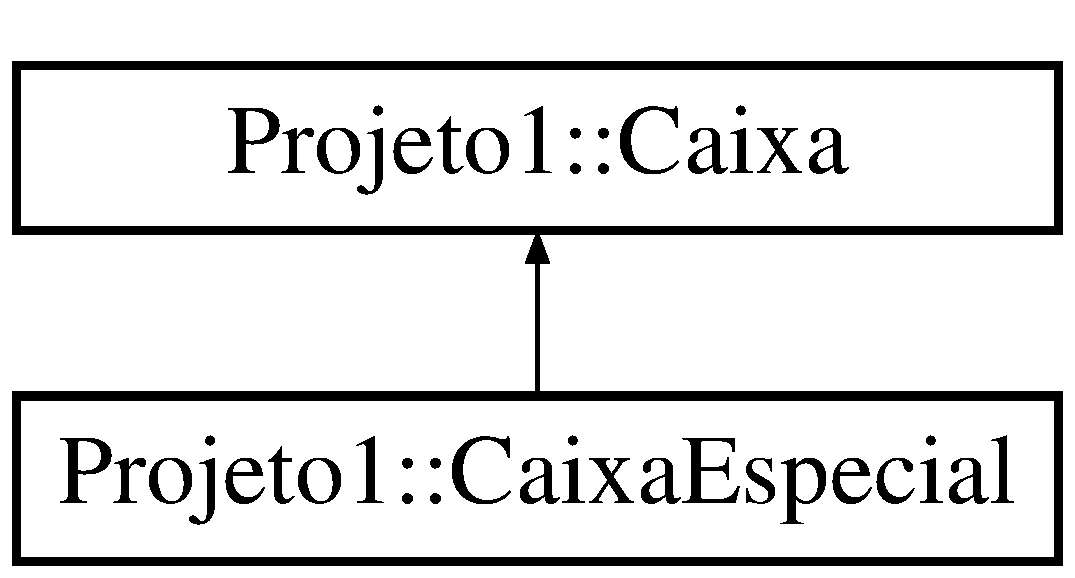
\includegraphics[height=2.000000cm]{classProjeto1_1_1Caixa}
\end{center}
\end{figure}
\subsection*{Public Member Functions}
\begin{DoxyCompactItemize}
\item 
\hyperlink{classProjeto1_1_1Caixa_ac54adc569decc044934b973b4066f82e}{Caixa} (char $\ast$nome, int \hyperlink{classProjeto1_1_1Caixa_aeb2c7dca9680e644f88f3bb9eb606c2a}{eficiencia}, int \hyperlink{classProjeto1_1_1Caixa_ad9f8c9b65400bd1db9004dbb3c9f18ea}{salario})
\item 
\hyperlink{classProjeto1_1_1Caixa_a3186951816b7bba0b473a97d1fc44565}{Caixa} ()
\item 
virtual \hyperlink{classProjeto1_1_1Caixa_a5860cd7dc1a6fb064f025b8cd24cc872}{$\sim$Caixa} ()
\item 
int \hyperlink{classProjeto1_1_1Caixa_a9501a2f8df6c4717db844327ac8c3a82}{enfileirar} (\hyperlink{classProjeto1_1_1Cliente}{Cliente} $\ast$dado)
\item 
\hyperlink{classProjeto1_1_1Cliente}{Cliente} $\ast$ \hyperlink{classProjeto1_1_1Caixa_a60a829984934de75e264bfebbebb56fb}{desenfileirar} ()
\item 
void \hyperlink{classProjeto1_1_1Caixa_a4363134abfee713c0d02f47510b4e93f}{limpar} ()
\item 
int \hyperlink{classProjeto1_1_1Caixa_a0492c45bba7b53805bfe322ec1e8b993}{receberCliente} (\hyperlink{classProjeto1_1_1Cliente}{Cliente} $\ast$cliente)
\item 
virtual int \hyperlink{classProjeto1_1_1Caixa_a70c900f948864a28e2661dab17b10f9f}{fornecaLucro} ()
\item 
long int \hyperlink{classProjeto1_1_1Caixa_af082f5059bce22f7ed3d72de9e6b0fad}{atenderCliente} (int horaAtual)
\item 
void \hyperlink{classProjeto1_1_1Caixa_ae4c5c43dfcbae9198ae70624505f74b5}{mostrar} ()
\item 
void \hyperlink{classProjeto1_1_1Caixa_af4a87b003b6be708d883908573b0f88a}{apresentarRelatorio} ()
\end{DoxyCompactItemize}
\subsection*{Public Attributes}
\begin{DoxyCompactItemize}
\item 
char $\ast$ \hyperlink{classProjeto1_1_1Caixa_a3396ba1f8fd63194ff225ffaf0d5268c}{nomeCaixa}
\item 
int \hyperlink{classProjeto1_1_1Caixa_aeb2c7dca9680e644f88f3bb9eb606c2a}{eficiencia}
\item 
int \hyperlink{classProjeto1_1_1Caixa_ad9f8c9b65400bd1db9004dbb3c9f18ea}{salario}
\item 
int \hyperlink{classProjeto1_1_1Caixa_ac836b24da5b62bd7d9382ada7d0222a4}{clientesAtendidos}
\item 
int \hyperlink{classProjeto1_1_1Caixa_a2a7071befa8bd345aae8bc42b9d08e24}{tempoMedio}
\item 
int \hyperlink{classProjeto1_1_1Caixa_aab5d05e900f913ed7d705bcb2c4e899d}{faturamentoTotal}
\item 
\hyperlink{classProjeto1_1_1ElementoDeFila}{ElementoDeFila} $\ast$ \hyperlink{classProjeto1_1_1Caixa_a81f31c6847218308e3285c385675c3d9}{primeiro}
\item 
\hyperlink{classProjeto1_1_1ElementoDeFila}{ElementoDeFila} $\ast$ \hyperlink{classProjeto1_1_1Caixa_adf2463f6ed9828bed7c3def83ab1fd95}{ultimo}
\item 
int \hyperlink{classProjeto1_1_1Caixa_a6a968db0d50c39f1429591190ad34791}{tamanhoFila}
\item 
int \hyperlink{classProjeto1_1_1Caixa_ab02cf6a92e30a62022a04335742f2767}{totalProdutos}
\end{DoxyCompactItemize}
\subsection*{Private Member Functions}
\begin{DoxyCompactItemize}
\item 
bool \hyperlink{classProjeto1_1_1Caixa_a099014e9d3fee7c7286ca347bc7955f6}{vazia} ()
\end{DoxyCompactItemize}


\subsection{Detailed Description}
Classe que representa um caixa de um supermercado. 

Definition at line 24 of file Caixa.h.



\subsection{Constructor \& Destructor Documentation}
\hypertarget{classProjeto1_1_1Caixa_ac54adc569decc044934b973b4066f82e}{
\index{Projeto1::Caixa@{Projeto1::Caixa}!Caixa@{Caixa}}
\index{Caixa@{Caixa}!Projeto1::Caixa@{Projeto1::Caixa}}
\subsubsection[{Caixa}]{\setlength{\rightskip}{0pt plus 5cm}Projeto1::Caixa::Caixa (
\begin{DoxyParamCaption}
\item[{char $\ast$}]{nome, }
\item[{int}]{eficienc, }
\item[{int}]{salari}
\end{DoxyParamCaption}
)}}
\label{classProjeto1_1_1Caixa_ac54adc569decc044934b973b4066f82e}
Construtor que gera um caixa de supermercado.


\begin{DoxyParams}{Parameters}
{\em nome} & : nome do operador do caixa. \\
\hline
{\em eficienc} & : eficiencia do operador do caixa. \\
\hline
{\em salari} & : salario do operador do caixa. \\
\hline
\end{DoxyParams}


Definition at line 20 of file Caixa.cpp.

\hypertarget{classProjeto1_1_1Caixa_a3186951816b7bba0b473a97d1fc44565}{
\index{Projeto1::Caixa@{Projeto1::Caixa}!Caixa@{Caixa}}
\index{Caixa@{Caixa}!Projeto1::Caixa@{Projeto1::Caixa}}
\subsubsection[{Caixa}]{\setlength{\rightskip}{0pt plus 5cm}Projeto1::Caixa::Caixa (
\begin{DoxyParamCaption}
{}
\end{DoxyParamCaption}
)}}
\label{classProjeto1_1_1Caixa_a3186951816b7bba0b473a97d1fc44565}


Definition at line 33 of file Caixa.cpp.

\hypertarget{classProjeto1_1_1Caixa_a5860cd7dc1a6fb064f025b8cd24cc872}{
\index{Projeto1::Caixa@{Projeto1::Caixa}!$\sim$Caixa@{$\sim$Caixa}}
\index{$\sim$Caixa@{$\sim$Caixa}!Projeto1::Caixa@{Projeto1::Caixa}}
\subsubsection[{$\sim$Caixa}]{\setlength{\rightskip}{0pt plus 5cm}Projeto1::Caixa::$\sim$Caixa (
\begin{DoxyParamCaption}
{}
\end{DoxyParamCaption}
)\hspace{0.3cm}{\ttfamily  \mbox{[}virtual\mbox{]}}}}
\label{classProjeto1_1_1Caixa_a5860cd7dc1a6fb064f025b8cd24cc872}
Destrutor que exclui um objeto da classe caixa. 

Definition at line 49 of file Caixa.cpp.



\subsection{Member Function Documentation}
\hypertarget{classProjeto1_1_1Caixa_af4a87b003b6be708d883908573b0f88a}{
\index{Projeto1::Caixa@{Projeto1::Caixa}!apresentarRelatorio@{apresentarRelatorio}}
\index{apresentarRelatorio@{apresentarRelatorio}!Projeto1::Caixa@{Projeto1::Caixa}}
\subsubsection[{apresentarRelatorio}]{\setlength{\rightskip}{0pt plus 5cm}void Projeto1::Caixa::apresentarRelatorio (
\begin{DoxyParamCaption}
{}
\end{DoxyParamCaption}
)}}
\label{classProjeto1_1_1Caixa_af4a87b003b6be708d883908573b0f88a}
Método que gera o relatório final da execução. 

Definition at line 212 of file Caixa.cpp.



Referenced by Projeto1::Supermercado::apresentarResultados().

\hypertarget{classProjeto1_1_1Caixa_af082f5059bce22f7ed3d72de9e6b0fad}{
\index{Projeto1::Caixa@{Projeto1::Caixa}!atenderCliente@{atenderCliente}}
\index{atenderCliente@{atenderCliente}!Projeto1::Caixa@{Projeto1::Caixa}}
\subsubsection[{atenderCliente}]{\setlength{\rightskip}{0pt plus 5cm}long int Projeto1::Caixa::atenderCliente (
\begin{DoxyParamCaption}
\item[{int}]{horaAtual}
\end{DoxyParamCaption}
)}}
\label{classProjeto1_1_1Caixa_af082f5059bce22f7ed3d72de9e6b0fad}
Método que verificar se o proximo cliente da fila deve ser atendimento.


\begin{DoxyParams}{Parameters}
{\em horaAtual} & : instante em que se encontra o programa. \\
\hline
\end{DoxyParams}
\begin{DoxyReturn}{Returns}
\hyperlink{classProjeto1_1_1Cliente}{Cliente} : cliente que foi atendido. 
\end{DoxyReturn}


Definition at line 193 of file Caixa.cpp.



Referenced by Projeto1::Supermercado::atenderClientes().

\hypertarget{classProjeto1_1_1Caixa_a60a829984934de75e264bfebbebb56fb}{
\index{Projeto1::Caixa@{Projeto1::Caixa}!desenfileirar@{desenfileirar}}
\index{desenfileirar@{desenfileirar}!Projeto1::Caixa@{Projeto1::Caixa}}
\subsubsection[{desenfileirar}]{\setlength{\rightskip}{0pt plus 5cm}{\bf Cliente} $\ast$ Projeto1::Caixa::desenfileirar (
\begin{DoxyParamCaption}
{}
\end{DoxyParamCaption}
)}}
\label{classProjeto1_1_1Caixa_a60a829984934de75e264bfebbebb56fb}
Método que remove um elemento da Fila. Primeiramente testa se a Fila possui elementos. Caso possua ele remove o primeiro elemento, ou seja o primeiro que foi inserido.

\begin{DoxyReturn}{Returns}
0(NULL) = caso a Fila não possua elementos. 

volta = ponteiro para um objeto da classe cliente. 
\end{DoxyReturn}


Definition at line 101 of file Caixa.cpp.



References Projeto1::ElementoDeFila::cliente, FILA\_\-VAZIA, and Projeto1::ElementoDeFila::proximo.

\hypertarget{classProjeto1_1_1Caixa_a9501a2f8df6c4717db844327ac8c3a82}{
\index{Projeto1::Caixa@{Projeto1::Caixa}!enfileirar@{enfileirar}}
\index{enfileirar@{enfileirar}!Projeto1::Caixa@{Projeto1::Caixa}}
\subsubsection[{enfileirar}]{\setlength{\rightskip}{0pt plus 5cm}int Projeto1::Caixa::enfileirar (
\begin{DoxyParamCaption}
\item[{{\bf Cliente} $\ast$}]{dado}
\end{DoxyParamCaption}
)}}
\label{classProjeto1_1_1Caixa_a9501a2f8df6c4717db844327ac8c3a82}
Método que adiciona um elemento da fila.

Primeiramente teste se ainda é possivel adicionar um elemento à fila. Caso isso não seja verdadeiro ele retorna uma constante FILA\_\-CHEIA.


\begin{DoxyParams}{Parameters}
{\em dado} & = ponteiro para um objeto da classe \hyperlink{classProjeto1_1_1Cliente}{Cliente}. \\
\hline
\end{DoxyParams}
\begin{DoxyReturn}{Returns}
FILA\_\-CHEIA = constante que representa a falta de espaço na Fila. 

tamanho = inteiro que informa a posição onde o dado foi inserido. 
\end{DoxyReturn}


Definition at line 63 of file Caixa.cpp.



References FILA\_\-CHEIA, and Projeto1::ElementoDeFila::proximo.

\hypertarget{classProjeto1_1_1Caixa_a70c900f948864a28e2661dab17b10f9f}{
\index{Projeto1::Caixa@{Projeto1::Caixa}!fornecaLucro@{fornecaLucro}}
\index{fornecaLucro@{fornecaLucro}!Projeto1::Caixa@{Projeto1::Caixa}}
\subsubsection[{fornecaLucro}]{\setlength{\rightskip}{0pt plus 5cm}int Projeto1::Caixa::fornecaLucro (
\begin{DoxyParamCaption}
{}
\end{DoxyParamCaption}
)\hspace{0.3cm}{\ttfamily  \mbox{[}virtual\mbox{]}}}}
\label{classProjeto1_1_1Caixa_a70c900f948864a28e2661dab17b10f9f}
Método que fornece o lucro gerado pelo caixa corrente.

\begin{DoxyReturn}{Returns}
lucro : ineiro. 
\end{DoxyReturn}


Reimplemented in \hyperlink{classProjeto1_1_1CaixaEspecial_a8b903f57784cc2f5025108db30939232}{Projeto1::CaixaEspecial}.



Definition at line 175 of file Caixa.cpp.



Referenced by Projeto1::Supermercado::apresentarResultados().

\hypertarget{classProjeto1_1_1Caixa_a4363134abfee713c0d02f47510b4e93f}{
\index{Projeto1::Caixa@{Projeto1::Caixa}!limpar@{limpar}}
\index{limpar@{limpar}!Projeto1::Caixa@{Projeto1::Caixa}}
\subsubsection[{limpar}]{\setlength{\rightskip}{0pt plus 5cm}void Projeto1::Caixa::limpar (
\begin{DoxyParamCaption}
{}
\end{DoxyParamCaption}
)}}
\label{classProjeto1_1_1Caixa_a4363134abfee713c0d02f47510b4e93f}
Método que exclui todos os elementos da fila e suas respectivas informações, representado pela classe \hyperlink{classProjeto1_1_1Cliente}{Cliente}. 

Definition at line 122 of file Caixa.cpp.



References Projeto1::ElementoDeFila::cliente, FILA\_\-VAZIA, and Projeto1::ElementoDeFila::proximo.

\hypertarget{classProjeto1_1_1Caixa_ae4c5c43dfcbae9198ae70624505f74b5}{
\index{Projeto1::Caixa@{Projeto1::Caixa}!mostrar@{mostrar}}
\index{mostrar@{mostrar}!Projeto1::Caixa@{Projeto1::Caixa}}
\subsubsection[{mostrar}]{\setlength{\rightskip}{0pt plus 5cm}void Projeto1::Caixa::mostrar (
\begin{DoxyParamCaption}
{}
\end{DoxyParamCaption}
)}}
\label{classProjeto1_1_1Caixa_ae4c5c43dfcbae9198ae70624505f74b5}
Método que imprime as informações do caixa. 

Definition at line 82 of file Caixa.cpp.

\hypertarget{classProjeto1_1_1Caixa_a0492c45bba7b53805bfe322ec1e8b993}{
\index{Projeto1::Caixa@{Projeto1::Caixa}!receberCliente@{receberCliente}}
\index{receberCliente@{receberCliente}!Projeto1::Caixa@{Projeto1::Caixa}}
\subsubsection[{receberCliente}]{\setlength{\rightskip}{0pt plus 5cm}int Projeto1::Caixa::receberCliente (
\begin{DoxyParamCaption}
\item[{{\bf Cliente} $\ast$}]{cliente}
\end{DoxyParamCaption}
)}}
\label{classProjeto1_1_1Caixa_a0492c45bba7b53805bfe322ec1e8b993}
Método que calcula o tempo de saida de um cliente de acordo com seus parâmetros e com a eficoência do caixa.


\begin{DoxyParams}{Parameters}
{\em cliente} & : cliente do supermercado. \\
\hline
\end{DoxyParams}


Definition at line 140 of file Caixa.cpp.



References Projeto1::Cliente::chegada, Projeto1::Cliente::cheque, Projeto1::Cliente::saida, and Projeto1::Cliente::totalCompras.



Referenced by Projeto1::Supermercado::posicionarCliente().

\hypertarget{classProjeto1_1_1Caixa_a099014e9d3fee7c7286ca347bc7955f6}{
\index{Projeto1::Caixa@{Projeto1::Caixa}!vazia@{vazia}}
\index{vazia@{vazia}!Projeto1::Caixa@{Projeto1::Caixa}}
\subsubsection[{vazia}]{\setlength{\rightskip}{0pt plus 5cm}bool Projeto1::Caixa::vazia (
\begin{DoxyParamCaption}
{}
\end{DoxyParamCaption}
)\hspace{0.3cm}{\ttfamily  \mbox{[}private\mbox{]}}}}
\label{classProjeto1_1_1Caixa_a099014e9d3fee7c7286ca347bc7955f6}
Metodo que testa se a fila possui elementos.

\begin{DoxyReturn}{Returns}
true = caso a Fila esteja vazia. 
\end{DoxyReturn}


Definition at line 90 of file Caixa.cpp.



References FILA\_\-VAZIA.



\subsection{Member Data Documentation}
\hypertarget{classProjeto1_1_1Caixa_ac836b24da5b62bd7d9382ada7d0222a4}{
\index{Projeto1::Caixa@{Projeto1::Caixa}!clientesAtendidos@{clientesAtendidos}}
\index{clientesAtendidos@{clientesAtendidos}!Projeto1::Caixa@{Projeto1::Caixa}}
\subsubsection[{clientesAtendidos}]{\setlength{\rightskip}{0pt plus 5cm}int {\bf Projeto1::Caixa::clientesAtendidos}}}
\label{classProjeto1_1_1Caixa_ac836b24da5b62bd7d9382ada7d0222a4}
numero de clientes atendidos 

Definition at line 37 of file Caixa.h.



Referenced by Projeto1::Supermercado::apresentarResultados().

\hypertarget{classProjeto1_1_1Caixa_aeb2c7dca9680e644f88f3bb9eb606c2a}{
\index{Projeto1::Caixa@{Projeto1::Caixa}!eficiencia@{eficiencia}}
\index{eficiencia@{eficiencia}!Projeto1::Caixa@{Projeto1::Caixa}}
\subsubsection[{eficiencia}]{\setlength{\rightskip}{0pt plus 5cm}int {\bf Projeto1::Caixa::eficiencia}}}
\label{classProjeto1_1_1Caixa_aeb2c7dca9680e644f88f3bb9eb606c2a}
eficiencia do caixa 

Definition at line 33 of file Caixa.h.

\hypertarget{classProjeto1_1_1Caixa_aab5d05e900f913ed7d705bcb2c4e899d}{
\index{Projeto1::Caixa@{Projeto1::Caixa}!faturamentoTotal@{faturamentoTotal}}
\index{faturamentoTotal@{faturamentoTotal}!Projeto1::Caixa@{Projeto1::Caixa}}
\subsubsection[{faturamentoTotal}]{\setlength{\rightskip}{0pt plus 5cm}int {\bf Projeto1::Caixa::faturamentoTotal}}}
\label{classProjeto1_1_1Caixa_aab5d05e900f913ed7d705bcb2c4e899d}
faturamento total 

Definition at line 41 of file Caixa.h.



Referenced by Projeto1::Supermercado::apresentarResultados(), and Projeto1::CaixaEspecial::fornecaLucro().

\hypertarget{classProjeto1_1_1Caixa_a3396ba1f8fd63194ff225ffaf0d5268c}{
\index{Projeto1::Caixa@{Projeto1::Caixa}!nomeCaixa@{nomeCaixa}}
\index{nomeCaixa@{nomeCaixa}!Projeto1::Caixa@{Projeto1::Caixa}}
\subsubsection[{nomeCaixa}]{\setlength{\rightskip}{0pt plus 5cm}char$\ast$ {\bf Projeto1::Caixa::nomeCaixa}}}
\label{classProjeto1_1_1Caixa_a3396ba1f8fd63194ff225ffaf0d5268c}
identificador do caixa 

Definition at line 31 of file Caixa.h.

\hypertarget{classProjeto1_1_1Caixa_a81f31c6847218308e3285c385675c3d9}{
\index{Projeto1::Caixa@{Projeto1::Caixa}!primeiro@{primeiro}}
\index{primeiro@{primeiro}!Projeto1::Caixa@{Projeto1::Caixa}}
\subsubsection[{primeiro}]{\setlength{\rightskip}{0pt plus 5cm}{\bf ElementoDeFila}$\ast$ {\bf Projeto1::Caixa::primeiro}}}
\label{classProjeto1_1_1Caixa_a81f31c6847218308e3285c385675c3d9}
FilaDeClientes 

Definition at line 45 of file Caixa.h.

\hypertarget{classProjeto1_1_1Caixa_ad9f8c9b65400bd1db9004dbb3c9f18ea}{
\index{Projeto1::Caixa@{Projeto1::Caixa}!salario@{salario}}
\index{salario@{salario}!Projeto1::Caixa@{Projeto1::Caixa}}
\subsubsection[{salario}]{\setlength{\rightskip}{0pt plus 5cm}int {\bf Projeto1::Caixa::salario}}}
\label{classProjeto1_1_1Caixa_ad9f8c9b65400bd1db9004dbb3c9f18ea}
salario do caixa 

Definition at line 35 of file Caixa.h.



Referenced by Projeto1::CaixaEspecial::fornecaLucro().

\hypertarget{classProjeto1_1_1Caixa_a6a968db0d50c39f1429591190ad34791}{
\index{Projeto1::Caixa@{Projeto1::Caixa}!tamanhoFila@{tamanhoFila}}
\index{tamanhoFila@{tamanhoFila}!Projeto1::Caixa@{Projeto1::Caixa}}
\subsubsection[{tamanhoFila}]{\setlength{\rightskip}{0pt plus 5cm}int {\bf Projeto1::Caixa::tamanhoFila}}}
\label{classProjeto1_1_1Caixa_a6a968db0d50c39f1429591190ad34791}
tamanho fila de clientes 

Definition at line 49 of file Caixa.h.



Referenced by Projeto1::Supermercado::chamarCaixaEspecial(), and Projeto1::Supermercado::posicionarCliente().

\hypertarget{classProjeto1_1_1Caixa_a2a7071befa8bd345aae8bc42b9d08e24}{
\index{Projeto1::Caixa@{Projeto1::Caixa}!tempoMedio@{tempoMedio}}
\index{tempoMedio@{tempoMedio}!Projeto1::Caixa@{Projeto1::Caixa}}
\subsubsection[{tempoMedio}]{\setlength{\rightskip}{0pt plus 5cm}int {\bf Projeto1::Caixa::tempoMedio}}}
\label{classProjeto1_1_1Caixa_a2a7071befa8bd345aae8bc42b9d08e24}
tempo medio de espera 

Definition at line 39 of file Caixa.h.

\hypertarget{classProjeto1_1_1Caixa_ab02cf6a92e30a62022a04335742f2767}{
\index{Projeto1::Caixa@{Projeto1::Caixa}!totalProdutos@{totalProdutos}}
\index{totalProdutos@{totalProdutos}!Projeto1::Caixa@{Projeto1::Caixa}}
\subsubsection[{totalProdutos}]{\setlength{\rightskip}{0pt plus 5cm}int {\bf Projeto1::Caixa::totalProdutos}}}
\label{classProjeto1_1_1Caixa_ab02cf6a92e30a62022a04335742f2767}
soma de todas as mercadorias dos clientes que estão na fila. 

Definition at line 51 of file Caixa.h.



Referenced by Projeto1::Supermercado::posicionarCliente().

\hypertarget{classProjeto1_1_1Caixa_adf2463f6ed9828bed7c3def83ab1fd95}{
\index{Projeto1::Caixa@{Projeto1::Caixa}!ultimo@{ultimo}}
\index{ultimo@{ultimo}!Projeto1::Caixa@{Projeto1::Caixa}}
\subsubsection[{ultimo}]{\setlength{\rightskip}{0pt plus 5cm}{\bf ElementoDeFila}$\ast$ {\bf Projeto1::Caixa::ultimo}}}
\label{classProjeto1_1_1Caixa_adf2463f6ed9828bed7c3def83ab1fd95}
FilaDeClientes 

Definition at line 47 of file Caixa.h.



The documentation for this class was generated from the following files:\begin{DoxyCompactItemize}
\item 
/home/will/Programming/C++/ED/Projeto 1/src/\hyperlink{Caixa_8h}{Caixa.h}\item 
/home/will/Programming/C++/ED/Projeto 1/src/\hyperlink{Caixa_8cpp}{Caixa.cpp}\end{DoxyCompactItemize}

\section{\-Projeto1\-:\-:\-Caixa\-Especial \-Class \-Reference}
\label{classProjeto1_1_1CaixaEspecial}\index{\-Projeto1\-::\-Caixa\-Especial@{\-Projeto1\-::\-Caixa\-Especial}}


{\ttfamily \#include $<$\-Caixa\-Especial.\-h$>$}

\-Inheritance diagram for \-Projeto1\-:\-:\-Caixa\-Especial\-:\begin{figure}[H]
\begin{center}
\leavevmode
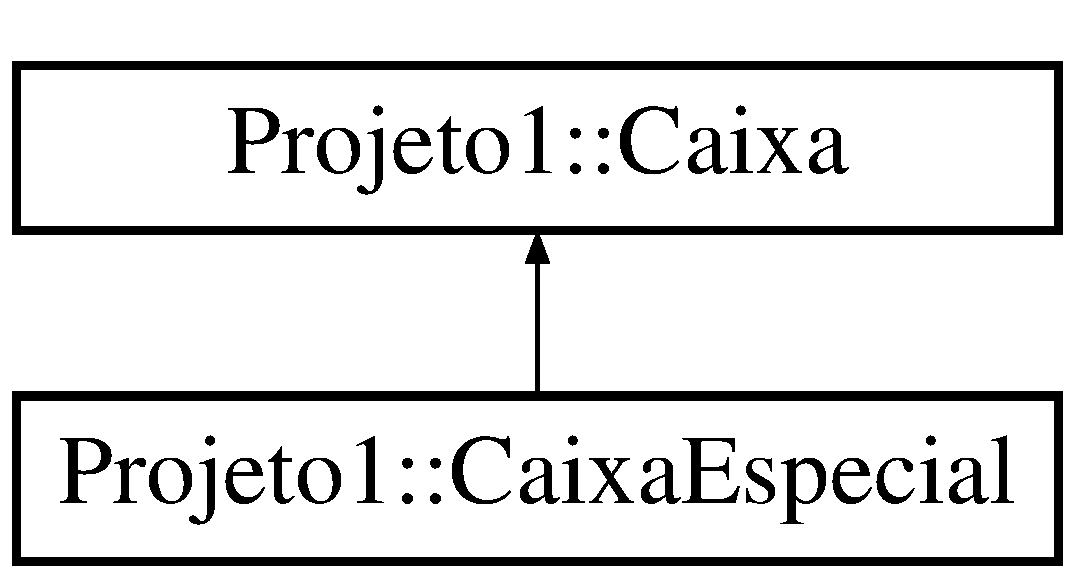
\includegraphics[height=2.000000cm]{classProjeto1_1_1CaixaEspecial}
\end{center}
\end{figure}
\subsection*{\-Public \-Member \-Functions}
\begin{DoxyCompactItemize}
\item 
{\bf \-Caixa\-Especial} (char $\ast$nome, int {\bf eficiencia}, int {\bf salario})
\item 
virtual int {\bf forneca\-Lucro} ()
\end{DoxyCompactItemize}


\subsection{\-Detailed \-Description}
\-Classe que representa um caixa em hora extra. 

\subsection{\-Constructor \& \-Destructor \-Documentation}
\index{\-Projeto1\-::\-Caixa\-Especial@{\-Projeto1\-::\-Caixa\-Especial}!\-Caixa\-Especial@{\-Caixa\-Especial}}
\index{\-Caixa\-Especial@{\-Caixa\-Especial}!Projeto1::CaixaEspecial@{\-Projeto1\-::\-Caixa\-Especial}}
\subsubsection[{\-Caixa\-Especial}]{\setlength{\rightskip}{0pt plus 5cm}{\bf \-Projeto1\-::\-Caixa\-Especial\-::\-Caixa\-Especial} (
\begin{DoxyParamCaption}
\item[{char $\ast$}]{nome, }
\item[{int}]{eficienc, }
\item[{int}]{salari}
\end{DoxyParamCaption}
)}\label{classProjeto1_1_1CaixaEspecial_aee786a831dd911aa2adef0bf232bb739}
\-Construtor que gera um caixa especial de supermercado.


\begin{DoxyParams}{\-Parameters}
{\em nome} & \-: nome do operador do caixa. \\
\hline
{\em eficienc} & \-: eficiencia do operador do caixa. \\
\hline
{\em salari} & \-: salario do operador do caixa. \\
\hline
\end{DoxyParams}


\subsection{\-Member \-Function \-Documentation}
\index{\-Projeto1\-::\-Caixa\-Especial@{\-Projeto1\-::\-Caixa\-Especial}!forneca\-Lucro@{forneca\-Lucro}}
\index{forneca\-Lucro@{forneca\-Lucro}!Projeto1::CaixaEspecial@{\-Projeto1\-::\-Caixa\-Especial}}
\subsubsection[{forneca\-Lucro}]{\setlength{\rightskip}{0pt plus 5cm}int {\bf \-Projeto1\-::\-Caixa\-Especial\-::forneca\-Lucro} (
\begin{DoxyParamCaption}
{}
\end{DoxyParamCaption}
)\hspace{0.3cm}{\ttfamily  [virtual]}}\label{classProjeto1_1_1CaixaEspecial_a8b903f57784cc2f5025108db30939232}
\-Método que fornece o lucro gerado pelo caixa durante a simulação.

\-Para tal fornecimento ele subtrai seu sálario, que é dobrado pois ele está em hora extra, de seu faturamento total.

\begin{DoxyReturn}{\-Returns}
lucro gerado pelo caixa. 
\end{DoxyReturn}


\-Reimplemented from {\bf \-Projeto1\-::\-Caixa} \doxyref{}{p.}{classProjeto1_1_1Caixa_a70c900f948864a28e2661dab17b10f9f}.



\-The documentation for this class was generated from the following files\-:\begin{DoxyCompactItemize}
\item 
src/\-Caixa\-Especial.\-h\item 
src/\-Caixa\-Especial.\-cpp\end{DoxyCompactItemize}

\section{\-Projeto1\-:\-:\-Cliente \-Class \-Reference}
\label{classProjeto1_1_1Cliente}\index{\-Projeto1\-::\-Cliente@{\-Projeto1\-::\-Cliente}}


{\ttfamily \#include $<$\-Cliente.\-h$>$}

\subsection*{\-Public \-Member \-Functions}
\begin{DoxyCompactItemize}
\item 
{\bf \-Cliente} (int {\bf chegada})
\item 
void {\bf gerar\-Total\-De\-Compras} ()
\item 
void {\bf calcular\-Valor\-De\-Compras} ()
\item 
void {\bf decidir\-Cheque} ()
\end{DoxyCompactItemize}
\subsection*{\-Public \-Attributes}
\begin{DoxyCompactItemize}
\item 
int {\bf total\-Compras}
\item 
int {\bf valor\-Compras}
\item 
int {\bf chegada}
\item 
int {\bf saida}
\item 
bool {\bf cheque}
\item 
\-Tipo\-Cliente {\bf tipo}
\end{DoxyCompactItemize}


\subsection{\-Detailed \-Description}
\-Classe que representa um cliente de um supermercado arbitrario. 

\subsection{\-Constructor \& \-Destructor \-Documentation}
\index{\-Projeto1\-::\-Cliente@{\-Projeto1\-::\-Cliente}!\-Cliente@{\-Cliente}}
\index{\-Cliente@{\-Cliente}!Projeto1::Cliente@{\-Projeto1\-::\-Cliente}}
\subsubsection[{\-Cliente}]{\setlength{\rightskip}{0pt plus 5cm}\-Projeto1\-::\-Cliente\-::\-Cliente (
\begin{DoxyParamCaption}
\item[{int}]{c}
\end{DoxyParamCaption}
)}\label{classProjeto1_1_1Cliente_a2753ad34ef32991f3ea25585d8a1fa8a}
\-Construtor que gera um objeto da classe \doxyref{\-Cliente}{p.}{classProjeto1_1_1Cliente}.


\begin{DoxyParams}{\-Parameters}
{\em c,\-:} & horario de chegada do cliente ao supermercado. \\
\hline
\end{DoxyParams}


\subsection{\-Member \-Function \-Documentation}
\index{\-Projeto1\-::\-Cliente@{\-Projeto1\-::\-Cliente}!calcular\-Valor\-De\-Compras@{calcular\-Valor\-De\-Compras}}
\index{calcular\-Valor\-De\-Compras@{calcular\-Valor\-De\-Compras}!Projeto1::Cliente@{\-Projeto1\-::\-Cliente}}
\subsubsection[{calcular\-Valor\-De\-Compras}]{\setlength{\rightskip}{0pt plus 5cm}void {\bf \-Projeto1\-::\-Cliente\-::calcular\-Valor\-De\-Compras} (
\begin{DoxyParamCaption}
{}
\end{DoxyParamCaption}
)}\label{classProjeto1_1_1Cliente_a6507e848da3d68d859663be187094efc}
\-Método que calcula o valor de cada compra do cliente.

\-Para isso ele usa o metodo \char`\"{}rand()\char`\"{}, que gera um numero aleatório,e delimita o intervalo de geração entre as constantes\-: \-M\-A\-X\-\_\-\-V\-A\-L\-O\-R e \-M\-I\-N\-\_\-\-V\-A\-L\-O\-R. \index{\-Projeto1\-::\-Cliente@{\-Projeto1\-::\-Cliente}!decidir\-Cheque@{decidir\-Cheque}}
\index{decidir\-Cheque@{decidir\-Cheque}!Projeto1::Cliente@{\-Projeto1\-::\-Cliente}}
\subsubsection[{decidir\-Cheque}]{\setlength{\rightskip}{0pt plus 5cm}void {\bf \-Projeto1\-::\-Cliente\-::decidir\-Cheque} (
\begin{DoxyParamCaption}
{}
\end{DoxyParamCaption}
)}\label{classProjeto1_1_1Cliente_a38c487a5b371ddef86d2b649b7f30872}
\-Método que gera a forma de pagamento de um cliente.

\-Para isso tem uma probabilidade de 20\% para pagamento em cheque e 80\% para dinheiro. \index{\-Projeto1\-::\-Cliente@{\-Projeto1\-::\-Cliente}!gerar\-Total\-De\-Compras@{gerar\-Total\-De\-Compras}}
\index{gerar\-Total\-De\-Compras@{gerar\-Total\-De\-Compras}!Projeto1::Cliente@{\-Projeto1\-::\-Cliente}}
\subsubsection[{gerar\-Total\-De\-Compras}]{\setlength{\rightskip}{0pt plus 5cm}void {\bf \-Projeto1\-::\-Cliente\-::gerar\-Total\-De\-Compras} (
\begin{DoxyParamCaption}
{}
\end{DoxyParamCaption}
)}\label{classProjeto1_1_1Cliente_af92320dc3f60493254a12d4295c842db}
\-Método que gera o npúmero total de compras de um cliente.

\-Para isso ele usa o metodo \char`\"{}rand()\char`\"{}, que gera um numero aleatório,e delimita o intervalo de geração entre as constantes\-: \-M\-A\-X\-\_\-\-C\-O\-M\-P\-R\-A\-S e \-M\-I\-N\-\_\-\-C\-O\-M\-P\-R\-A\-S. 

\subsection{\-Member \-Data \-Documentation}
\index{\-Projeto1\-::\-Cliente@{\-Projeto1\-::\-Cliente}!chegada@{chegada}}
\index{chegada@{chegada}!Projeto1::Cliente@{\-Projeto1\-::\-Cliente}}
\subsubsection[{chegada}]{\setlength{\rightskip}{0pt plus 5cm}int {\bf \-Projeto1\-::\-Cliente\-::chegada}}\label{classProjeto1_1_1Cliente_adc19105b9deaa9411028a32ba1eec9fc}
horario de chegada do cliente \index{\-Projeto1\-::\-Cliente@{\-Projeto1\-::\-Cliente}!cheque@{cheque}}
\index{cheque@{cheque}!Projeto1::Cliente@{\-Projeto1\-::\-Cliente}}
\subsubsection[{cheque}]{\setlength{\rightskip}{0pt plus 5cm}bool {\bf \-Projeto1\-::\-Cliente\-::cheque}}\label{classProjeto1_1_1Cliente_ad54c6376c859c8cdb68887b3948e9841}
\-True quando for pagamento em cheque \index{\-Projeto1\-::\-Cliente@{\-Projeto1\-::\-Cliente}!saida@{saida}}
\index{saida@{saida}!Projeto1::Cliente@{\-Projeto1\-::\-Cliente}}
\subsubsection[{saida}]{\setlength{\rightskip}{0pt plus 5cm}int {\bf \-Projeto1\-::\-Cliente\-::saida}}\label{classProjeto1_1_1Cliente_a868b7d7e3b824aed35511c433801824a}
horario de saida do cliente \index{\-Projeto1\-::\-Cliente@{\-Projeto1\-::\-Cliente}!tipo@{tipo}}
\index{tipo@{tipo}!Projeto1::Cliente@{\-Projeto1\-::\-Cliente}}
\subsubsection[{tipo}]{\setlength{\rightskip}{0pt plus 5cm}\-Tipo\-Cliente {\bf \-Projeto1\-::\-Cliente\-::tipo}}\label{classProjeto1_1_1Cliente_af37da5fe48856223d53932cf61d4b3f7}
enum de tipo do cliente \index{\-Projeto1\-::\-Cliente@{\-Projeto1\-::\-Cliente}!total\-Compras@{total\-Compras}}
\index{total\-Compras@{total\-Compras}!Projeto1::Cliente@{\-Projeto1\-::\-Cliente}}
\subsubsection[{total\-Compras}]{\setlength{\rightskip}{0pt plus 5cm}int {\bf \-Projeto1\-::\-Cliente\-::total\-Compras}}\label{classProjeto1_1_1Cliente_ae6670b6e5ba64ee23f9798845df586a5}
entre 2 e 100 \index{\-Projeto1\-::\-Cliente@{\-Projeto1\-::\-Cliente}!valor\-Compras@{valor\-Compras}}
\index{valor\-Compras@{valor\-Compras}!Projeto1::Cliente@{\-Projeto1\-::\-Cliente}}
\subsubsection[{valor\-Compras}]{\setlength{\rightskip}{0pt plus 5cm}int {\bf \-Projeto1\-::\-Cliente\-::valor\-Compras}}\label{classProjeto1_1_1Cliente_a37b32637d513c756c817415f618d8d9d}
cada item varia entre 1 e 90r\$ dai td junto é colocado aqui 

\-The documentation for this class was generated from the following files\-:\begin{DoxyCompactItemize}
\item 
src/\-Cliente.\-h\item 
src/\-Cliente.\-cpp\end{DoxyCompactItemize}

\hypertarget{classProjeto1_1_1ElementoDeFila}{
\section{Projeto1::ElementoDeFila Class Reference}
\label{classProjeto1_1_1ElementoDeFila}\index{Projeto1::ElementoDeFila@{Projeto1::ElementoDeFila}}
}


{\ttfamily \#include $<$ElementoDeFila.h$>$}

\subsection*{Public Member Functions}
\begin{DoxyCompactItemize}
\item 
\hyperlink{classProjeto1_1_1ElementoDeFila_a04c2a994dcd9c959645e1973edbdece1}{ElementoDeFila} ()
\item 
\hyperlink{classProjeto1_1_1ElementoDeFila_aade4aa1072f2467b3bfd4c6474c87faa}{ElementoDeFila} (\hyperlink{classProjeto1_1_1Cliente}{Cliente} $\ast$info)
\item 
virtual \hyperlink{classProjeto1_1_1ElementoDeFila_ab01575efe125553a2024453032654fd5}{$\sim$ElementoDeFila} ()
\end{DoxyCompactItemize}
\subsection*{Public Attributes}
\begin{DoxyCompactItemize}
\item 
\hyperlink{classProjeto1_1_1ElementoDeFila}{ElementoDeFila} $\ast$ \hyperlink{classProjeto1_1_1ElementoDeFila_a2ca3828f86b949959b03c3f0986434c8}{proximo}
\item 
\hyperlink{classProjeto1_1_1Cliente}{Cliente} $\ast$ \hyperlink{classProjeto1_1_1ElementoDeFila_a5a75508f83800ff9eded46dc6fdfc71f}{cliente}
\end{DoxyCompactItemize}


\subsection{Detailed Description}
Classe que representa um objeto pertencente a uma lista genérica. 

Definition at line 18 of file ElementoDeFila.h.



\subsection{Constructor \& Destructor Documentation}
\hypertarget{classProjeto1_1_1ElementoDeFila_a04c2a994dcd9c959645e1973edbdece1}{
\index{Projeto1::ElementoDeFila@{Projeto1::ElementoDeFila}!ElementoDeFila@{ElementoDeFila}}
\index{ElementoDeFila@{ElementoDeFila}!Projeto1::ElementoDeFila@{Projeto1::ElementoDeFila}}
\subsubsection[{ElementoDeFila}]{\setlength{\rightskip}{0pt plus 5cm}Projeto1::ElementoDeFila::ElementoDeFila (
\begin{DoxyParamCaption}
{}
\end{DoxyParamCaption}
)}}
\label{classProjeto1_1_1ElementoDeFila_a04c2a994dcd9c959645e1973edbdece1}
Método que constrói um objeto que representa uma elemento de uma fila encadeado. 

Definition at line 16 of file ElementoDeFila.cpp.

\hypertarget{classProjeto1_1_1ElementoDeFila_aade4aa1072f2467b3bfd4c6474c87faa}{
\index{Projeto1::ElementoDeFila@{Projeto1::ElementoDeFila}!ElementoDeFila@{ElementoDeFila}}
\index{ElementoDeFila@{ElementoDeFila}!Projeto1::ElementoDeFila@{Projeto1::ElementoDeFila}}
\subsubsection[{ElementoDeFila}]{\setlength{\rightskip}{0pt plus 5cm}Projeto1::ElementoDeFila::ElementoDeFila (
\begin{DoxyParamCaption}
\item[{{\bf Cliente} $\ast$}]{inf}
\end{DoxyParamCaption}
)}}
\label{classProjeto1_1_1ElementoDeFila_aade4aa1072f2467b3bfd4c6474c87faa}
Método que constrói um objeto que representa uma elemento de uma fila encadeado. 
\begin{DoxyParams}{Parameters}
{\em inf} & : ponteiro para um objeto da classe \hyperlink{classProjeto1_1_1Cliente}{Cliente}. \\
\hline
\end{DoxyParams}


Definition at line 25 of file ElementoDeFila.cpp.



References cliente.

\hypertarget{classProjeto1_1_1ElementoDeFila_ab01575efe125553a2024453032654fd5}{
\index{Projeto1::ElementoDeFila@{Projeto1::ElementoDeFila}!$\sim$ElementoDeFila@{$\sim$ElementoDeFila}}
\index{$\sim$ElementoDeFila@{$\sim$ElementoDeFila}!Projeto1::ElementoDeFila@{Projeto1::ElementoDeFila}}
\subsubsection[{$\sim$ElementoDeFila}]{\setlength{\rightskip}{0pt plus 5cm}Projeto1::ElementoDeFila::$\sim$ElementoDeFila (
\begin{DoxyParamCaption}
{}
\end{DoxyParamCaption}
)\hspace{0.3cm}{\ttfamily  \mbox{[}virtual\mbox{]}}}}
\label{classProjeto1_1_1ElementoDeFila_ab01575efe125553a2024453032654fd5}
Destrutor que exclui um elemento da Fila. 

Definition at line 33 of file ElementoDeFila.cpp.



\subsection{Member Data Documentation}
\hypertarget{classProjeto1_1_1ElementoDeFila_a5a75508f83800ff9eded46dc6fdfc71f}{
\index{Projeto1::ElementoDeFila@{Projeto1::ElementoDeFila}!cliente@{cliente}}
\index{cliente@{cliente}!Projeto1::ElementoDeFila@{Projeto1::ElementoDeFila}}
\subsubsection[{cliente}]{\setlength{\rightskip}{0pt plus 5cm}{\bf Cliente}$\ast$ {\bf Projeto1::ElementoDeFila::cliente}}}
\label{classProjeto1_1_1ElementoDeFila_a5a75508f83800ff9eded46dc6fdfc71f}
Ponteiro para o cliente referente a este elemento da fila. 

Definition at line 26 of file ElementoDeFila.h.



Referenced by Projeto1::Caixa::desenfileirar(), ElementoDeFila(), and Projeto1::Caixa::limpar().

\hypertarget{classProjeto1_1_1ElementoDeFila_a2ca3828f86b949959b03c3f0986434c8}{
\index{Projeto1::ElementoDeFila@{Projeto1::ElementoDeFila}!proximo@{proximo}}
\index{proximo@{proximo}!Projeto1::ElementoDeFila@{Projeto1::ElementoDeFila}}
\subsubsection[{proximo}]{\setlength{\rightskip}{0pt plus 5cm}{\bf ElementoDeFila}$\ast$ {\bf Projeto1::ElementoDeFila::proximo}}}
\label{classProjeto1_1_1ElementoDeFila_a2ca3828f86b949959b03c3f0986434c8}
Proximo cliente da fila do caixa 

Definition at line 24 of file ElementoDeFila.h.



Referenced by Projeto1::Caixa::desenfileirar(), Projeto1::Caixa::enfileirar(), and Projeto1::Caixa::limpar().



The documentation for this class was generated from the following files:\begin{DoxyCompactItemize}
\item 
/home/will/Programming/C++/ED/Projeto 1/src/\hyperlink{ElementoDeFila_8h}{ElementoDeFila.h}\item 
/home/will/Programming/C++/ED/Projeto 1/src/\hyperlink{ElementoDeFila_8cpp}{ElementoDeFila.cpp}\end{DoxyCompactItemize}

\section{\-Projeto1\-:\-:\-Elemento\-De\-Lista\-Circular \-Class \-Reference}
\label{classProjeto1_1_1ElementoDeListaCircular}\index{\-Projeto1\-::\-Elemento\-De\-Lista\-Circular@{\-Projeto1\-::\-Elemento\-De\-Lista\-Circular}}


{\ttfamily \#include $<$\-Elemento\-Da\-Lista\-Circular.\-h$>$}

\subsection*{\-Public \-Member \-Functions}
\begin{DoxyCompactItemize}
\item 
{\bf \-Elemento\-De\-Lista\-Circular} ({\bf \-Caixa} $\ast${\bf caixa})
\item 
virtual {\bf $\sim$\-Elemento\-De\-Lista\-Circular} ()
\end{DoxyCompactItemize}
\subsection*{\-Public \-Attributes}
\begin{DoxyCompactItemize}
\item 
{\bf \-Elemento\-De\-Lista\-Circular} $\ast$ {\bf proximo}
\item 
{\bf \-Caixa} $\ast$ {\bf caixa}
\end{DoxyCompactItemize}


\subsection{\-Detailed \-Description}
\-Representação de um objeto que será integrado à \-Lista. 

\subsection{\-Constructor \& \-Destructor \-Documentation}
\index{\-Projeto1\-::\-Elemento\-De\-Lista\-Circular@{\-Projeto1\-::\-Elemento\-De\-Lista\-Circular}!\-Elemento\-De\-Lista\-Circular@{\-Elemento\-De\-Lista\-Circular}}
\index{\-Elemento\-De\-Lista\-Circular@{\-Elemento\-De\-Lista\-Circular}!Projeto1::ElementoDeListaCircular@{\-Projeto1\-::\-Elemento\-De\-Lista\-Circular}}
\subsubsection[{\-Elemento\-De\-Lista\-Circular}]{\setlength{\rightskip}{0pt plus 5cm}\-Projeto1\-::\-Elemento\-De\-Lista\-Circular\-::\-Elemento\-De\-Lista\-Circular (
\begin{DoxyParamCaption}
\item[{{\bf \-Caixa} $\ast$}]{c}
\end{DoxyParamCaption}
)}\label{classProjeto1_1_1ElementoDeListaCircular_a25516bba2a32834a346ccb08a9b40cc2}
\-Construtor que configura um objeto da classe \-Elemento\-De\-Lista.


\begin{DoxyParams}{\-Parameters}
{\em c} & \-: ponteiro para um objeto da classe \doxyref{\-Caixa}{p.}{classProjeto1_1_1Caixa}. \\
\hline
\end{DoxyParams}
\index{\-Projeto1\-::\-Elemento\-De\-Lista\-Circular@{\-Projeto1\-::\-Elemento\-De\-Lista\-Circular}!$\sim$\-Elemento\-De\-Lista\-Circular@{$\sim$\-Elemento\-De\-Lista\-Circular}}
\index{$\sim$\-Elemento\-De\-Lista\-Circular@{$\sim$\-Elemento\-De\-Lista\-Circular}!Projeto1::ElementoDeListaCircular@{\-Projeto1\-::\-Elemento\-De\-Lista\-Circular}}
\subsubsection[{$\sim$\-Elemento\-De\-Lista\-Circular}]{\setlength{\rightskip}{0pt plus 5cm}{\bf \-Projeto1\-::\-Elemento\-De\-Lista\-Circular\-::$\sim$\-Elemento\-De\-Lista\-Circular} (
\begin{DoxyParamCaption}
{}
\end{DoxyParamCaption}
)\hspace{0.3cm}{\ttfamily  [virtual]}}\label{classProjeto1_1_1ElementoDeListaCircular_a659b6674090be47acb2be96bcecd65ce}
\-Destrutoer que exclui um objeto da classe \-Elemento\-De\-Lista. 

\subsection{\-Member \-Data \-Documentation}
\index{\-Projeto1\-::\-Elemento\-De\-Lista\-Circular@{\-Projeto1\-::\-Elemento\-De\-Lista\-Circular}!caixa@{caixa}}
\index{caixa@{caixa}!Projeto1::ElementoDeListaCircular@{\-Projeto1\-::\-Elemento\-De\-Lista\-Circular}}
\subsubsection[{caixa}]{\setlength{\rightskip}{0pt plus 5cm}{\bf \-Caixa}$\ast$ {\bf \-Projeto1\-::\-Elemento\-De\-Lista\-Circular\-::caixa}}\label{classProjeto1_1_1ElementoDeListaCircular_a814668b406a3835016a372b5069bb822}
\-Ponteiro para o caixa referente a este elemento de lista. \index{\-Projeto1\-::\-Elemento\-De\-Lista\-Circular@{\-Projeto1\-::\-Elemento\-De\-Lista\-Circular}!proximo@{proximo}}
\index{proximo@{proximo}!Projeto1::ElementoDeListaCircular@{\-Projeto1\-::\-Elemento\-De\-Lista\-Circular}}
\subsubsection[{proximo}]{\setlength{\rightskip}{0pt plus 5cm}{\bf \-Elemento\-De\-Lista\-Circular}$\ast$ {\bf \-Projeto1\-::\-Elemento\-De\-Lista\-Circular\-::proximo}}\label{classProjeto1_1_1ElementoDeListaCircular_a65b5ca20f12c1436d2ffa96421be919b}
\-Proximo caixa da lista de caixas 

\-The documentation for this class was generated from the following files\-:\begin{DoxyCompactItemize}
\item 
src/\-Elemento\-Da\-Lista\-Circular.\-h\item 
src/\-Elemento\-Da\-Lista\-Circular.\-cpp\end{DoxyCompactItemize}

\section{\-Projeto1\-:\-:\-Lista\-Circular \-Class \-Reference}
\label{classProjeto1_1_1ListaCircular}\index{\-Projeto1\-::\-Lista\-Circular@{\-Projeto1\-::\-Lista\-Circular}}


{\ttfamily \#include $<$\-Lista\-Circular.\-h$>$}

\subsection*{\-Public \-Member \-Functions}
\begin{DoxyCompactItemize}
\item 
{\bf \-Lista\-Circular} ()
\item 
virtual {\bf $\sim$\-Lista\-Circular} ()
\item 
int {\bf adiciona} ({\bf \-Caixa} $\ast$caixa)
\item 
void {\bf mostrar\-Lista} ()
\end{DoxyCompactItemize}
\subsection*{\-Public \-Attributes}
\begin{DoxyCompactItemize}
\item 
{\bf \-Elemento\-De\-Lista\-Circular} $\ast$ {\bf sentinela}
\item 
int {\bf tamanho}
\end{DoxyCompactItemize}


\subsection{\-Detailed \-Description}
\-Classe que modela uma lista encadeada.

\-Uma lista encadeada ou lista ligada é uma estrutura de dados linear e dinâmica. \-Ela é composta por células que apontam para o próximo elemento da lista. \-Para \char`\"{}ter\char`\"{} uma lista ligada/encadeada, basta guardar seu primeiro elemento, e seu último elemento aponta para uma célula nula.\par
 \-Para mais informações acesse\-:\par
 {\tt http\-://pt.\-wikipedia.\-org/wiki/\-Lista\-\_\-ligada} 

\subsection{\-Constructor \& \-Destructor \-Documentation}
\index{\-Projeto1\-::\-Lista\-Circular@{\-Projeto1\-::\-Lista\-Circular}!\-Lista\-Circular@{\-Lista\-Circular}}
\index{\-Lista\-Circular@{\-Lista\-Circular}!Projeto1::ListaCircular@{\-Projeto1\-::\-Lista\-Circular}}
\subsubsection[{\-Lista\-Circular}]{\setlength{\rightskip}{0pt plus 5cm}{\bf \-Projeto1\-::\-Lista\-Circular\-::\-Lista\-Circular} (
\begin{DoxyParamCaption}
{}
\end{DoxyParamCaption}
)}\label{classProjeto1_1_1ListaCircular_ad1f1e2d58ba59c3b20d926dbee0bd68a}
\-Método que constri um objeto que representa uma lista encadeada. \index{\-Projeto1\-::\-Lista\-Circular@{\-Projeto1\-::\-Lista\-Circular}!$\sim$\-Lista\-Circular@{$\sim$\-Lista\-Circular}}
\index{$\sim$\-Lista\-Circular@{$\sim$\-Lista\-Circular}!Projeto1::ListaCircular@{\-Projeto1\-::\-Lista\-Circular}}
\subsubsection[{$\sim$\-Lista\-Circular}]{\setlength{\rightskip}{0pt plus 5cm}{\bf \-Projeto1\-::\-Lista\-Circular\-::$\sim$\-Lista\-Circular} (
\begin{DoxyParamCaption}
{}
\end{DoxyParamCaption}
)\hspace{0.3cm}{\ttfamily  [virtual]}}\label{classProjeto1_1_1ListaCircular_afcca3f790d99dc9c747d03414612c4eb}
\-Destrutor que exclui uma lista encadeada.

\-Para isso utiliza o método limpar. 

\subsection{\-Member \-Function \-Documentation}
\index{\-Projeto1\-::\-Lista\-Circular@{\-Projeto1\-::\-Lista\-Circular}!adiciona@{adiciona}}
\index{adiciona@{adiciona}!Projeto1::ListaCircular@{\-Projeto1\-::\-Lista\-Circular}}
\subsubsection[{adiciona}]{\setlength{\rightskip}{0pt plus 5cm}int {\bf \-Projeto1\-::\-Lista\-Circular\-::adiciona} (
\begin{DoxyParamCaption}
\item[{{\bf \-Caixa} $\ast$}]{caixa}
\end{DoxyParamCaption}
)}\label{classProjeto1_1_1ListaCircular_a35dc09255c50dd5c1fbdc80ba84b1b55}
\-Método que adiciona no início um objeto da classe \-Elemento\-De\-Lista.

\-Para isso verifica se ha espaço na mesma. \-Caso a questão anterior seja verdadeira o objeto é adicionado na primeira posição da \-Lista.


\begin{DoxyParams}{\-Parameters}
{\em caixa} & \-: ponteiro para o caixa onde o cliente vai ser inserido.\\
\hline
\end{DoxyParams}
\begin{DoxyReturn}{\-Returns}
\-L\-I\-S\-R\-A\-\_\-\-C\-H\-E\-I\-A = constante que representa a falta de espaço na \-Lista. 

1 = inteiro que informa a posição onde o dado foi inserido. 
\end{DoxyReturn}
\index{\-Projeto1\-::\-Lista\-Circular@{\-Projeto1\-::\-Lista\-Circular}!mostrar\-Lista@{mostrar\-Lista}}
\index{mostrar\-Lista@{mostrar\-Lista}!Projeto1::ListaCircular@{\-Projeto1\-::\-Lista\-Circular}}
\subsubsection[{mostrar\-Lista}]{\setlength{\rightskip}{0pt plus 5cm}void {\bf \-Projeto1\-::\-Lista\-Circular\-::mostrar\-Lista} (
\begin{DoxyParamCaption}
{}
\end{DoxyParamCaption}
)}\label{classProjeto1_1_1ListaCircular_a17fb0d61349d4898cbdeb9e86e004759}
\-Método que imprime a \-Lista no console. 

\subsection{\-Member \-Data \-Documentation}
\index{\-Projeto1\-::\-Lista\-Circular@{\-Projeto1\-::\-Lista\-Circular}!sentinela@{sentinela}}
\index{sentinela@{sentinela}!Projeto1::ListaCircular@{\-Projeto1\-::\-Lista\-Circular}}
\subsubsection[{sentinela}]{\setlength{\rightskip}{0pt plus 5cm}{\bf \-Elemento\-De\-Lista\-Circular}$\ast$ {\bf \-Projeto1\-::\-Lista\-Circular\-::sentinela}}\label{classProjeto1_1_1ListaCircular_a20d805843e5fd2b012db44ad1e705472}
\-Primeiro elemento da lista circular. \index{\-Projeto1\-::\-Lista\-Circular@{\-Projeto1\-::\-Lista\-Circular}!tamanho@{tamanho}}
\index{tamanho@{tamanho}!Projeto1::ListaCircular@{\-Projeto1\-::\-Lista\-Circular}}
\subsubsection[{tamanho}]{\setlength{\rightskip}{0pt plus 5cm}int {\bf \-Projeto1\-::\-Lista\-Circular\-::tamanho}}\label{classProjeto1_1_1ListaCircular_a56720f9fadf008f0a0ba3eac4fb6e52b}
\-Tamanho da lista circular 

\-The documentation for this class was generated from the following files\-:\begin{DoxyCompactItemize}
\item 
src/\-Lista\-Circular.\-h\item 
src/\-Lista\-Circular.\-cpp\end{DoxyCompactItemize}

\hypertarget{classProjeto1_1_1Supermercado}{
\section{Projeto1::Supermercado Class Reference}
\label{classProjeto1_1_1Supermercado}\index{Projeto1::Supermercado@{Projeto1::Supermercado}}
}


{\ttfamily \#include $<$Supermercado.h$>$}

\subsection*{Public Member Functions}
\begin{DoxyCompactItemize}
\item 
\hyperlink{classProjeto1_1_1Supermercado_a712c285ce22c7b4cd0f4982484fcb092}{Supermercado} ()
\item 
\hyperlink{classProjeto1_1_1Supermercado_abb21b74f59b760e1e020bd706ad317ce}{Supermercado} (\hyperlink{classProjeto1_1_1ListaCircular}{ListaCircular} $\ast$\hyperlink{classProjeto1_1_1Supermercado_a0377fe11973f887d33fc7c743dd499de}{caixas}, int tempClientes, int tempoTotal)
\item 
virtual \hyperlink{classProjeto1_1_1Supermercado_a45e97c3a5c1b125fb2ad826270ba29eb}{$\sim$Supermercado} ()
\item 
void \hyperlink{classProjeto1_1_1Supermercado_a95984fac6635ea22f660e4038266b132}{iniciarSimulacao} ()
\item 
\hyperlink{classProjeto1_1_1Cliente}{Cliente} $\ast$ \hyperlink{classProjeto1_1_1Supermercado_a8182c122d2b8141f34c423762433c4f2}{gerarCliente} (int horario)
\item 
int \hyperlink{classProjeto1_1_1Supermercado_a006f42c2ab267236c96c5037230dd43a}{posicionarCliente} (\hyperlink{classProjeto1_1_1Cliente}{Cliente} $\ast$novo)
\item 
int \hyperlink{classProjeto1_1_1Supermercado_a7f998920216d84164f1feeda811aa7a4}{atenderClientes} (int horario)
\item 
void \hyperlink{classProjeto1_1_1Supermercado_a9e2055bab0973293e53c24154256a126}{chamarCaixaEspecial} ()
\item 
void \hyperlink{classProjeto1_1_1Supermercado_a918550e12e3f815b5aff5b5449886342}{configurarSimulacao} (char $\ast$nome, int \hyperlink{classProjeto1_1_1Supermercado_a6ec7501178b500d6a82330c99f95867e}{tempoSimulacao}, int \hyperlink{Main_8cpp_a0b097839315eb6a33ba1e11ce290fc9b}{tempoMedioChegada}, int \hyperlink{classProjeto1_1_1Supermercado_a11e5d386fe154d3e8ee3d8f7fa3d28a1}{limiteCaixaEspecial}, \hyperlink{classProjeto1_1_1ListaCircular}{ListaCircular} $\ast$\hyperlink{classProjeto1_1_1Supermercado_a0377fe11973f887d33fc7c743dd499de}{caixas})
\item 
void \hyperlink{classProjeto1_1_1Supermercado_a1c5c7fba6e33df1e597a2ab446dd5dd7}{apresentarResultados} ()
\end{DoxyCompactItemize}
\subsection*{Public Attributes}
\begin{DoxyCompactItemize}
\item 
\hyperlink{classProjeto1_1_1ListaCircular}{ListaCircular} $\ast$ \hyperlink{classProjeto1_1_1Supermercado_a0377fe11973f887d33fc7c743dd499de}{caixas}
\item 
char $\ast$ \hyperlink{classProjeto1_1_1Supermercado_a05fc2f885e22cf0d109d921d0f386baa}{nomeSupermercado}
\item 
int \hyperlink{classProjeto1_1_1Supermercado_a91df73523b452afac103edea5862f651}{tempoMedioClientes}
\item 
int \hyperlink{classProjeto1_1_1Supermercado_a6ec7501178b500d6a82330c99f95867e}{tempoSimulacao}
\item 
int \hyperlink{classProjeto1_1_1Supermercado_a258d2c48df71a1827f83e2658aa1e26d}{desistencias}
\item 
int \hyperlink{classProjeto1_1_1Supermercado_adcecd89e129cf0486b6ce02d162c4a55}{faturamentoBruto}
\item 
int \hyperlink{classProjeto1_1_1Supermercado_af210ce3a01e004c464d8abb03c74fedc}{valorDesistencias}
\item 
int \hyperlink{classProjeto1_1_1Supermercado_a11e5d386fe154d3e8ee3d8f7fa3d28a1}{limiteCaixaEspecial}
\item 
bool \hyperlink{classProjeto1_1_1Supermercado_a5e49476334361f1d056f5394a517a763}{caixaEspecialchamado}
\end{DoxyCompactItemize}


\subsection{Detailed Description}


Definition at line 15 of file Supermercado.h.



\subsection{Constructor \& Destructor Documentation}
\hypertarget{classProjeto1_1_1Supermercado_a712c285ce22c7b4cd0f4982484fcb092}{
\index{Projeto1::Supermercado@{Projeto1::Supermercado}!Supermercado@{Supermercado}}
\index{Supermercado@{Supermercado}!Projeto1::Supermercado@{Projeto1::Supermercado}}
\subsubsection[{Supermercado}]{\setlength{\rightskip}{0pt plus 5cm}Projeto1::Supermercado::Supermercado (
\begin{DoxyParamCaption}
{}
\end{DoxyParamCaption}
)}}
\label{classProjeto1_1_1Supermercado_a712c285ce22c7b4cd0f4982484fcb092}
Costrutor que gera um objeto da classe supermercado. 

Definition at line 21 of file Supermercado.cpp.



References caixas, limiteCaixaEspecial, and tempoSimulacao.

\hypertarget{classProjeto1_1_1Supermercado_abb21b74f59b760e1e020bd706ad317ce}{
\index{Projeto1::Supermercado@{Projeto1::Supermercado}!Supermercado@{Supermercado}}
\index{Supermercado@{Supermercado}!Projeto1::Supermercado@{Projeto1::Supermercado}}
\subsubsection[{Supermercado}]{\setlength{\rightskip}{0pt plus 5cm}Projeto1::Supermercado::Supermercado (
\begin{DoxyParamCaption}
\item[{{\bf ListaCircular} $\ast$}]{c, }
\item[{int}]{tempClientes, }
\item[{int}]{tempoTotal}
\end{DoxyParamCaption}
)}}
\label{classProjeto1_1_1Supermercado_abb21b74f59b760e1e020bd706ad317ce}
Costrutor que gera um objeto da classe supermercado.


\begin{DoxyParams}{Parameters}
{\em c} & : Pponteiro para Lista Circular de caixas do supermercado. \\
\hline
{\em tempClientes} & : Tempo médio de chegada de clientes. \\
\hline
{\em tempoTotal} & : Tempo total da simulação. \\
\hline
\end{DoxyParams}


Definition at line 37 of file Supermercado.cpp.



References caixas, limiteCaixaEspecial, and tempoSimulacao.

\hypertarget{classProjeto1_1_1Supermercado_a45e97c3a5c1b125fb2ad826270ba29eb}{
\index{Projeto1::Supermercado@{Projeto1::Supermercado}!$\sim$Supermercado@{$\sim$Supermercado}}
\index{$\sim$Supermercado@{$\sim$Supermercado}!Projeto1::Supermercado@{Projeto1::Supermercado}}
\subsubsection[{$\sim$Supermercado}]{\setlength{\rightskip}{0pt plus 5cm}Projeto1::Supermercado::$\sim$Supermercado (
\begin{DoxyParamCaption}
{}
\end{DoxyParamCaption}
)\hspace{0.3cm}{\ttfamily  \mbox{[}virtual\mbox{]}}}}
\label{classProjeto1_1_1Supermercado_a45e97c3a5c1b125fb2ad826270ba29eb}


Definition at line 46 of file Supermercado.cpp.



\subsection{Member Function Documentation}
\hypertarget{classProjeto1_1_1Supermercado_a1c5c7fba6e33df1e597a2ab446dd5dd7}{
\index{Projeto1::Supermercado@{Projeto1::Supermercado}!apresentarResultados@{apresentarResultados}}
\index{apresentarResultados@{apresentarResultados}!Projeto1::Supermercado@{Projeto1::Supermercado}}
\subsubsection[{apresentarResultados}]{\setlength{\rightskip}{0pt plus 5cm}void Projeto1::Supermercado::apresentarResultados (
\begin{DoxyParamCaption}
{}
\end{DoxyParamCaption}
)}}
\label{classProjeto1_1_1Supermercado_a1c5c7fba6e33df1e597a2ab446dd5dd7}
Método que gera os resultados finais da execução. 

Definition at line 198 of file Supermercado.cpp.



References Projeto1::Caixa::apresentarRelatorio(), Projeto1::ElementoDeListaCircular::caixa, caixas, Projeto1::Caixa::clientesAtendidos, Projeto1::Caixa::faturamentoTotal, Projeto1::Caixa::fornecaLucro(), nomeSupermercado, Projeto1::ElementoDeListaCircular::proximo, Projeto1::ListaCircular::sentinela, Projeto1::ListaCircular::tamanho, and tempoSimulacao.



Referenced by main().

\hypertarget{classProjeto1_1_1Supermercado_a7f998920216d84164f1feeda811aa7a4}{
\index{Projeto1::Supermercado@{Projeto1::Supermercado}!atenderClientes@{atenderClientes}}
\index{atenderClientes@{atenderClientes}!Projeto1::Supermercado@{Projeto1::Supermercado}}
\subsubsection[{atenderClientes}]{\setlength{\rightskip}{0pt plus 5cm}int Projeto1::Supermercado::atenderClientes (
\begin{DoxyParamCaption}
\item[{int}]{horario}
\end{DoxyParamCaption}
)}}
\label{classProjeto1_1_1Supermercado_a7f998920216d84164f1feeda811aa7a4}
Método que atended um cliente.

Para isso ele percorre todos os caixas e verifica se o primeiro cliente da fila deve ser atendido, ou seja, se o tempo de saida desse cliente é igual ao tempo atual de execução.


\begin{DoxyParams}{Parameters}
{\em horario} & : hora atual de execução. \\
\hline
\end{DoxyParams}


Definition at line 162 of file Supermercado.cpp.



References Projeto1::Caixa::atenderCliente(), Projeto1::ElementoDeListaCircular::caixa, caixas, Projeto1::ElementoDeListaCircular::proximo, and Projeto1::ListaCircular::sentinela.

\hypertarget{classProjeto1_1_1Supermercado_a9e2055bab0973293e53c24154256a126}{
\index{Projeto1::Supermercado@{Projeto1::Supermercado}!chamarCaixaEspecial@{chamarCaixaEspecial}}
\index{chamarCaixaEspecial@{chamarCaixaEspecial}!Projeto1::Supermercado@{Projeto1::Supermercado}}
\subsubsection[{chamarCaixaEspecial}]{\setlength{\rightskip}{0pt plus 5cm}void Projeto1::Supermercado::chamarCaixaEspecial (
\begin{DoxyParamCaption}
{}
\end{DoxyParamCaption}
)}}
\label{classProjeto1_1_1Supermercado_a9e2055bab0973293e53c24154256a126}
Método que chama (constrói) um caixa do tipo caixa expecial. 

Definition at line 174 of file Supermercado.cpp.



References Projeto1::ListaCircular::adiciona(), Projeto1::ElementoDeListaCircular::caixa, caixas, limiteCaixaEspecial, Projeto1::ElementoDeListaCircular::proximo, Projeto1::ListaCircular::sentinela, and Projeto1::Caixa::tamanhoFila.

\hypertarget{classProjeto1_1_1Supermercado_a918550e12e3f815b5aff5b5449886342}{
\index{Projeto1::Supermercado@{Projeto1::Supermercado}!configurarSimulacao@{configurarSimulacao}}
\index{configurarSimulacao@{configurarSimulacao}!Projeto1::Supermercado@{Projeto1::Supermercado}}
\subsubsection[{configurarSimulacao}]{\setlength{\rightskip}{0pt plus 5cm}void Projeto1::Supermercado::configurarSimulacao (
\begin{DoxyParamCaption}
\item[{char $\ast$}]{nome, }
\item[{int}]{tempoS, }
\item[{int}]{tempoMedioC, }
\item[{int}]{limiteCaixaEsp, }
\item[{{\bf ListaCircular} $\ast$}]{c}
\end{DoxyParamCaption}
)}}
\label{classProjeto1_1_1Supermercado_a918550e12e3f815b5aff5b5449886342}
Método que configura a simulação.


\begin{DoxyParams}{Parameters}
{\em nome} & : nome do supermercado. \\
\hline
{\em tempoS} & : tempo de simulação. \\
\hline
{\em tempoMedioC} & : tempo médio de chegada de clientes. \\
\hline
{\em limiteCaixaEsp,:} & limite de todas as filas antes de chamar o \hyperlink{classProjeto1_1_1Caixa}{Caixa} Especial \\
\hline
{\em c} & : lista de caixas; \\
\hline
\end{DoxyParams}


Definition at line 58 of file Supermercado.cpp.



References caixas, limiteCaixaEspecial, nomeSupermercado, and tempoSimulacao.



Referenced by main().

\hypertarget{classProjeto1_1_1Supermercado_a8182c122d2b8141f34c423762433c4f2}{
\index{Projeto1::Supermercado@{Projeto1::Supermercado}!gerarCliente@{gerarCliente}}
\index{gerarCliente@{gerarCliente}!Projeto1::Supermercado@{Projeto1::Supermercado}}
\subsubsection[{gerarCliente}]{\setlength{\rightskip}{0pt plus 5cm}{\bf Cliente} $\ast$ Projeto1::Supermercado::gerarCliente (
\begin{DoxyParamCaption}
\item[{int}]{horario}
\end{DoxyParamCaption}
)}}
\label{classProjeto1_1_1Supermercado_a8182c122d2b8141f34c423762433c4f2}
Método que gera um cliente do supremercado, decidindo o tipo do mesmo.

Existem dois tipos de clientes, os que buscam a fila com menos clientes e os que buscam uma fila com menor numero de produtos dos outros clientes. 

Definition at line 97 of file Supermercado.cpp.



References Projeto1::BuscaFilaComMenosProdutos, Projeto1::BuscaMenorFila, and Projeto1::Cliente::tipo.

\hypertarget{classProjeto1_1_1Supermercado_a95984fac6635ea22f660e4038266b132}{
\index{Projeto1::Supermercado@{Projeto1::Supermercado}!iniciarSimulacao@{iniciarSimulacao}}
\index{iniciarSimulacao@{iniciarSimulacao}!Projeto1::Supermercado@{Projeto1::Supermercado}}
\subsubsection[{iniciarSimulacao}]{\setlength{\rightskip}{0pt plus 5cm}void Projeto1::Supermercado::iniciarSimulacao (
\begin{DoxyParamCaption}
{}
\end{DoxyParamCaption}
)}}
\label{classProjeto1_1_1Supermercado_a95984fac6635ea22f660e4038266b132}
Método que executa a simulação.

Para isso percorre segundo a segundo executando os passos da simulação. 

Definition at line 71 of file Supermercado.cpp.



References tempoSimulacao.



Referenced by main().

\hypertarget{classProjeto1_1_1Supermercado_a006f42c2ab267236c96c5037230dd43a}{
\index{Projeto1::Supermercado@{Projeto1::Supermercado}!posicionarCliente@{posicionarCliente}}
\index{posicionarCliente@{posicionarCliente}!Projeto1::Supermercado@{Projeto1::Supermercado}}
\subsubsection[{posicionarCliente}]{\setlength{\rightskip}{0pt plus 5cm}int Projeto1::Supermercado::posicionarCliente (
\begin{DoxyParamCaption}
\item[{{\bf Cliente} $\ast$}]{novo}
\end{DoxyParamCaption}
)}}
\label{classProjeto1_1_1Supermercado_a006f42c2ab267236c96c5037230dd43a}
Método que posiciona um cliente na fila de um caixa, de acordo com seu tipo.


\begin{DoxyParams}{Parameters}
{\em novo} & : \hyperlink{classProjeto1_1_1Cliente}{Cliente} a ser posicionado. \\
\hline
\end{DoxyParams}


Definition at line 111 of file Supermercado.cpp.



References Projeto1::BuscaFilaComMenosProdutos, Projeto1::BuscaMenorFila, Projeto1::ElementoDeListaCircular::caixa, caixas, FATOR\_\-IRRITACAO, MAX\_\-CAIXA, Projeto1::ElementoDeListaCircular::proximo, Projeto1::Caixa::receberCliente(), Projeto1::ListaCircular::sentinela, Projeto1::Caixa::tamanhoFila, Projeto1::Cliente::tipo, Projeto1::Caixa::totalProdutos, and Projeto1::Cliente::valorCompras.



\subsection{Member Data Documentation}
\hypertarget{classProjeto1_1_1Supermercado_a5e49476334361f1d056f5394a517a763}{
\index{Projeto1::Supermercado@{Projeto1::Supermercado}!caixaEspecialchamado@{caixaEspecialchamado}}
\index{caixaEspecialchamado@{caixaEspecialchamado}!Projeto1::Supermercado@{Projeto1::Supermercado}}
\subsubsection[{caixaEspecialchamado}]{\setlength{\rightskip}{0pt plus 5cm}bool {\bf Projeto1::Supermercado::caixaEspecialchamado}}}
\label{classProjeto1_1_1Supermercado_a5e49476334361f1d056f5394a517a763}
Informação se um caixa especial já foi chamado. 

Definition at line 37 of file Supermercado.h.

\hypertarget{classProjeto1_1_1Supermercado_a0377fe11973f887d33fc7c743dd499de}{
\index{Projeto1::Supermercado@{Projeto1::Supermercado}!caixas@{caixas}}
\index{caixas@{caixas}!Projeto1::Supermercado@{Projeto1::Supermercado}}
\subsubsection[{caixas}]{\setlength{\rightskip}{0pt plus 5cm}{\bf ListaCircular}$\ast$ {\bf Projeto1::Supermercado::caixas}}}
\label{classProjeto1_1_1Supermercado_a0377fe11973f887d33fc7c743dd499de}
Lista de caixas. 

Definition at line 21 of file Supermercado.h.

\hypertarget{classProjeto1_1_1Supermercado_a258d2c48df71a1827f83e2658aa1e26d}{
\index{Projeto1::Supermercado@{Projeto1::Supermercado}!desistencias@{desistencias}}
\index{desistencias@{desistencias}!Projeto1::Supermercado@{Projeto1::Supermercado}}
\subsubsection[{desistencias}]{\setlength{\rightskip}{0pt plus 5cm}int {\bf Projeto1::Supermercado::desistencias}}}
\label{classProjeto1_1_1Supermercado_a258d2c48df71a1827f83e2658aa1e26d}
Número de clientes que desistiram. 

Definition at line 29 of file Supermercado.h.

\hypertarget{classProjeto1_1_1Supermercado_adcecd89e129cf0486b6ce02d162c4a55}{
\index{Projeto1::Supermercado@{Projeto1::Supermercado}!faturamentoBruto@{faturamentoBruto}}
\index{faturamentoBruto@{faturamentoBruto}!Projeto1::Supermercado@{Projeto1::Supermercado}}
\subsubsection[{faturamentoBruto}]{\setlength{\rightskip}{0pt plus 5cm}int {\bf Projeto1::Supermercado::faturamentoBruto}}}
\label{classProjeto1_1_1Supermercado_adcecd89e129cf0486b6ce02d162c4a55}
Faturamento bruto do supermercado. 

Definition at line 31 of file Supermercado.h.

\hypertarget{classProjeto1_1_1Supermercado_a11e5d386fe154d3e8ee3d8f7fa3d28a1}{
\index{Projeto1::Supermercado@{Projeto1::Supermercado}!limiteCaixaEspecial@{limiteCaixaEspecial}}
\index{limiteCaixaEspecial@{limiteCaixaEspecial}!Projeto1::Supermercado@{Projeto1::Supermercado}}
\subsubsection[{limiteCaixaEspecial}]{\setlength{\rightskip}{0pt plus 5cm}int {\bf Projeto1::Supermercado::limiteCaixaEspecial}}}
\label{classProjeto1_1_1Supermercado_a11e5d386fe154d3e8ee3d8f7fa3d28a1}
Limite para chamar um caixa especial. 

Definition at line 35 of file Supermercado.h.

\hypertarget{classProjeto1_1_1Supermercado_a05fc2f885e22cf0d109d921d0f386baa}{
\index{Projeto1::Supermercado@{Projeto1::Supermercado}!nomeSupermercado@{nomeSupermercado}}
\index{nomeSupermercado@{nomeSupermercado}!Projeto1::Supermercado@{Projeto1::Supermercado}}
\subsubsection[{nomeSupermercado}]{\setlength{\rightskip}{0pt plus 5cm}char$\ast$ {\bf Projeto1::Supermercado::nomeSupermercado}}}
\label{classProjeto1_1_1Supermercado_a05fc2f885e22cf0d109d921d0f386baa}
Nome do supermercado. 

Definition at line 23 of file Supermercado.h.

\hypertarget{classProjeto1_1_1Supermercado_a91df73523b452afac103edea5862f651}{
\index{Projeto1::Supermercado@{Projeto1::Supermercado}!tempoMedioClientes@{tempoMedioClientes}}
\index{tempoMedioClientes@{tempoMedioClientes}!Projeto1::Supermercado@{Projeto1::Supermercado}}
\subsubsection[{tempoMedioClientes}]{\setlength{\rightskip}{0pt plus 5cm}int {\bf Projeto1::Supermercado::tempoMedioClientes}}}
\label{classProjeto1_1_1Supermercado_a91df73523b452afac103edea5862f651}
Tempo medio de chegada de clientes. 

Definition at line 25 of file Supermercado.h.

\hypertarget{classProjeto1_1_1Supermercado_a6ec7501178b500d6a82330c99f95867e}{
\index{Projeto1::Supermercado@{Projeto1::Supermercado}!tempoSimulacao@{tempoSimulacao}}
\index{tempoSimulacao@{tempoSimulacao}!Projeto1::Supermercado@{Projeto1::Supermercado}}
\subsubsection[{tempoSimulacao}]{\setlength{\rightskip}{0pt plus 5cm}int {\bf Projeto1::Supermercado::tempoSimulacao}}}
\label{classProjeto1_1_1Supermercado_a6ec7501178b500d6a82330c99f95867e}
Tempo de Simulação. 

Definition at line 27 of file Supermercado.h.

\hypertarget{classProjeto1_1_1Supermercado_af210ce3a01e004c464d8abb03c74fedc}{
\index{Projeto1::Supermercado@{Projeto1::Supermercado}!valorDesistencias@{valorDesistencias}}
\index{valorDesistencias@{valorDesistencias}!Projeto1::Supermercado@{Projeto1::Supermercado}}
\subsubsection[{valorDesistencias}]{\setlength{\rightskip}{0pt plus 5cm}int {\bf Projeto1::Supermercado::valorDesistencias}}}
\label{classProjeto1_1_1Supermercado_af210ce3a01e004c464d8abb03c74fedc}
Prejuiso gerado pelas desistências. 

Definition at line 33 of file Supermercado.h.



The documentation for this class was generated from the following files:\begin{DoxyCompactItemize}
\item 
/home/will/Programming/C++/ED/Projeto 1/src/\hyperlink{Supermercado_8h}{Supermercado.h}\item 
/home/will/Programming/C++/ED/Projeto 1/src/\hyperlink{Supermercado_8cpp}{Supermercado.cpp}\end{DoxyCompactItemize}

\chapter{File Documentation}
\hypertarget{Caixa_8cpp}{
\section{/home/will/Programming/C++/ED/Projeto 1/src/Caixa.cpp File Reference}
\label{Caixa_8cpp}\index{/home/will/Programming/C++/ED/Projeto 1/src/Caixa.cpp@{/home/will/Programming/C++/ED/Projeto 1/src/Caixa.cpp}}
}
{\ttfamily \#include $<$iostream$>$}\par
{\ttfamily \#include $<$fstream$>$}\par
{\ttfamily \#include \char`\"{}Caixa.h\char`\"{}}\par
\subsection*{Namespaces}
\begin{DoxyCompactItemize}
\item 
namespace \hyperlink{namespaceProjeto1}{Projeto1}
\end{DoxyCompactItemize}

\hypertarget{Caixa_8h}{
\section{/home/will/Programming/C++/ED/Projeto 1/src/Caixa.h File Reference}
\label{Caixa_8h}\index{/home/will/Programming/C++/ED/Projeto 1/src/Caixa.h@{/home/will/Programming/C++/ED/Projeto 1/src/Caixa.h}}
}
{\ttfamily \#include $<$iostream$>$}\par
{\ttfamily \#include $<$fstream$>$}\par
{\ttfamily \#include \char`\"{}ElementoDeFila.h\char`\"{}}\par
\subsection*{Classes}
\begin{DoxyCompactItemize}
\item 
class \hyperlink{classProjeto1_1_1Caixa}{Projeto1::Caixa}
\end{DoxyCompactItemize}
\subsection*{Namespaces}
\begin{DoxyCompactItemize}
\item 
namespace \hyperlink{namespaceProjeto1}{Projeto1}
\end{DoxyCompactItemize}
\subsection*{Defines}
\begin{DoxyCompactItemize}
\item 
\#define \hyperlink{Caixa_8h_a5405bf1a7d136d94e6415fc0c8db02ca}{FILA\_\-VAZIA}~0
\item 
\#define \hyperlink{Caixa_8h_aee8549164da3c74cdcdd0f8794d2192f}{FILA\_\-CHEIA}~-\/2
\item 
\#define \hyperlink{Caixa_8h_a1bf8cb7a5bf30e7ccc1bbd7d1e9fe675}{ERRO\_\-POSICAO}~-\/3
\end{DoxyCompactItemize}


\subsection{Define Documentation}
\hypertarget{Caixa_8h_a1bf8cb7a5bf30e7ccc1bbd7d1e9fe675}{
\index{Caixa.h@{Caixa.h}!ERRO\_\-POSICAO@{ERRO\_\-POSICAO}}
\index{ERRO\_\-POSICAO@{ERRO\_\-POSICAO}!Caixa.h@{Caixa.h}}
\subsubsection[{ERRO\_\-POSICAO}]{\setlength{\rightskip}{0pt plus 5cm}\#define ERRO\_\-POSICAO~-\/3}}
\label{Caixa_8h_a1bf8cb7a5bf30e7ccc1bbd7d1e9fe675}


Definition at line 14 of file Caixa.h.

\hypertarget{Caixa_8h_aee8549164da3c74cdcdd0f8794d2192f}{
\index{Caixa.h@{Caixa.h}!FILA\_\-CHEIA@{FILA\_\-CHEIA}}
\index{FILA\_\-CHEIA@{FILA\_\-CHEIA}!Caixa.h@{Caixa.h}}
\subsubsection[{FILA\_\-CHEIA}]{\setlength{\rightskip}{0pt plus 5cm}\#define FILA\_\-CHEIA~-\/2}}
\label{Caixa_8h_aee8549164da3c74cdcdd0f8794d2192f}


Definition at line 13 of file Caixa.h.



Referenced by Projeto1::Caixa::enfileirar().

\hypertarget{Caixa_8h_a5405bf1a7d136d94e6415fc0c8db02ca}{
\index{Caixa.h@{Caixa.h}!FILA\_\-VAZIA@{FILA\_\-VAZIA}}
\index{FILA\_\-VAZIA@{FILA\_\-VAZIA}!Caixa.h@{Caixa.h}}
\subsubsection[{FILA\_\-VAZIA}]{\setlength{\rightskip}{0pt plus 5cm}\#define FILA\_\-VAZIA~0}}
\label{Caixa_8h_a5405bf1a7d136d94e6415fc0c8db02ca}


Definition at line 12 of file Caixa.h.



Referenced by Projeto1::Caixa::desenfileirar(), Projeto1::Caixa::limpar(), and Projeto1::Caixa::vazia().


\hypertarget{CaixaEspecial_8cpp}{
\section{/home/will/Programming/C++/ED/Projeto 1/src/CaixaEspecial.cpp File Reference}
\label{CaixaEspecial_8cpp}\index{/home/will/Programming/C++/ED/Projeto 1/src/CaixaEspecial.cpp@{/home/will/Programming/C++/ED/Projeto 1/src/CaixaEspecial.cpp}}
}
{\ttfamily \#include \char`\"{}CaixaEspecial.h\char`\"{}}\par
\subsection*{Namespaces}
\begin{DoxyCompactItemize}
\item 
namespace \hyperlink{namespaceProjeto1}{Projeto1}
\end{DoxyCompactItemize}

\hypertarget{CaixaEspecial_8h}{
\section{/home/will/Programming/C++/ED/Projeto 1/src/CaixaEspecial.h File Reference}
\label{CaixaEspecial_8h}\index{/home/will/Programming/C++/ED/Projeto 1/src/CaixaEspecial.h@{/home/will/Programming/C++/ED/Projeto 1/src/CaixaEspecial.h}}
}
{\ttfamily \#include \char`\"{}Caixa.h\char`\"{}}\par
\subsection*{Classes}
\begin{DoxyCompactItemize}
\item 
class \hyperlink{classProjeto1_1_1CaixaEspecial}{Projeto1::CaixaEspecial}
\end{DoxyCompactItemize}
\subsection*{Namespaces}
\begin{DoxyCompactItemize}
\item 
namespace \hyperlink{namespaceProjeto1}{Projeto1}
\end{DoxyCompactItemize}

\hypertarget{Cliente_8cpp}{
\section{/home/will/Programming/C++/ED/Projeto 1/src/Cliente.cpp File Reference}
\label{Cliente_8cpp}\index{/home/will/Programming/C++/ED/Projeto 1/src/Cliente.cpp@{/home/will/Programming/C++/ED/Projeto 1/src/Cliente.cpp}}
}
{\ttfamily \#include \char`\"{}Cliente.h\char`\"{}}\par
{\ttfamily \#include $<$cstdlib$>$}\par
{\ttfamily \#include $<$stdio.h$>$}\par
{\ttfamily \#include $<$iostream$>$}\par
{\ttfamily \#include $<$time.h$>$}\par
\subsection*{Namespaces}
\begin{DoxyCompactItemize}
\item 
namespace \hyperlink{namespaceProjeto1}{Projeto1}
\end{DoxyCompactItemize}

\hypertarget{Cliente_8h}{
\section{/home/will/Programming/C++/ED/Projeto 1/src/Cliente.h File Reference}
\label{Cliente_8h}\index{/home/will/Programming/C++/ED/Projeto 1/src/Cliente.h@{/home/will/Programming/C++/ED/Projeto 1/src/Cliente.h}}
}
\subsection*{Classes}
\begin{DoxyCompactItemize}
\item 
class \hyperlink{classProjeto1_1_1Cliente}{Projeto1::Cliente}
\end{DoxyCompactItemize}
\subsection*{Namespaces}
\begin{DoxyCompactItemize}
\item 
namespace \hyperlink{namespaceProjeto1}{Projeto1}
\end{DoxyCompactItemize}
\subsection*{Defines}
\begin{DoxyCompactItemize}
\item 
\#define \hyperlink{Cliente_8h_aee1f448022017953eaced50c10f9931d}{MIN\_\-COMPRAS}~2
\item 
\#define \hyperlink{Cliente_8h_aeeee8d17eab56b83a65e5dd775817b33}{MAX\_\-COMPRAS}~100
\item 
\#define \hyperlink{Cliente_8h_a63a24ec2eff17e030f5f37e6d2992338}{MIN\_\-VALOR}~1
\item 
\#define \hyperlink{Cliente_8h_afe11496592057bdce8c76e909867110b}{MAX\_\-VALOR}~90
\item 
\#define \hyperlink{Cliente_8h_ae98f088daaa68e53d3a689c1007b88f6}{PROB\_\-CHEQUE}~20
\end{DoxyCompactItemize}
\subsection*{Enumerations}
\begin{DoxyCompactItemize}
\item 
enum \hyperlink{namespaceProjeto1_a4dade362b39c779d6411abf4ba19aeed}{Projeto1::TipoCliente} \{ \hyperlink{namespaceProjeto1_a4dade362b39c779d6411abf4ba19aeeda3c2a34a5670e3315f0c5493a00890611}{Projeto1::BuscaMenorFila}, 
\hyperlink{namespaceProjeto1_a4dade362b39c779d6411abf4ba19aeedaec1ed9ba7657b9ea20b55bada08f1825}{Projeto1::BuscaFilaComMenosProdutos}
 \}
\end{DoxyCompactItemize}


\subsection{Define Documentation}
\hypertarget{Cliente_8h_aeeee8d17eab56b83a65e5dd775817b33}{
\index{Cliente.h@{Cliente.h}!MAX\_\-COMPRAS@{MAX\_\-COMPRAS}}
\index{MAX\_\-COMPRAS@{MAX\_\-COMPRAS}!Cliente.h@{Cliente.h}}
\subsubsection[{MAX\_\-COMPRAS}]{\setlength{\rightskip}{0pt plus 5cm}\#define MAX\_\-COMPRAS~100}}
\label{Cliente_8h_aeeee8d17eab56b83a65e5dd775817b33}


Definition at line 11 of file Cliente.h.



Referenced by Projeto1::Cliente::gerarTotalDeCompras().

\hypertarget{Cliente_8h_afe11496592057bdce8c76e909867110b}{
\index{Cliente.h@{Cliente.h}!MAX\_\-VALOR@{MAX\_\-VALOR}}
\index{MAX\_\-VALOR@{MAX\_\-VALOR}!Cliente.h@{Cliente.h}}
\subsubsection[{MAX\_\-VALOR}]{\setlength{\rightskip}{0pt plus 5cm}\#define MAX\_\-VALOR~90}}
\label{Cliente_8h_afe11496592057bdce8c76e909867110b}


Definition at line 13 of file Cliente.h.



Referenced by Projeto1::Cliente::calcularValorDeCompras(), and Projeto1::Cliente::gerarTotalDeCompras().

\hypertarget{Cliente_8h_aee1f448022017953eaced50c10f9931d}{
\index{Cliente.h@{Cliente.h}!MIN\_\-COMPRAS@{MIN\_\-COMPRAS}}
\index{MIN\_\-COMPRAS@{MIN\_\-COMPRAS}!Cliente.h@{Cliente.h}}
\subsubsection[{MIN\_\-COMPRAS}]{\setlength{\rightskip}{0pt plus 5cm}\#define MIN\_\-COMPRAS~2}}
\label{Cliente_8h_aee1f448022017953eaced50c10f9931d}


Definition at line 10 of file Cliente.h.



Referenced by Projeto1::Cliente::gerarTotalDeCompras().

\hypertarget{Cliente_8h_a63a24ec2eff17e030f5f37e6d2992338}{
\index{Cliente.h@{Cliente.h}!MIN\_\-VALOR@{MIN\_\-VALOR}}
\index{MIN\_\-VALOR@{MIN\_\-VALOR}!Cliente.h@{Cliente.h}}
\subsubsection[{MIN\_\-VALOR}]{\setlength{\rightskip}{0pt plus 5cm}\#define MIN\_\-VALOR~1}}
\label{Cliente_8h_a63a24ec2eff17e030f5f37e6d2992338}


Definition at line 12 of file Cliente.h.



Referenced by Projeto1::Cliente::calcularValorDeCompras(), and Projeto1::Cliente::gerarTotalDeCompras().

\hypertarget{Cliente_8h_ae98f088daaa68e53d3a689c1007b88f6}{
\index{Cliente.h@{Cliente.h}!PROB\_\-CHEQUE@{PROB\_\-CHEQUE}}
\index{PROB\_\-CHEQUE@{PROB\_\-CHEQUE}!Cliente.h@{Cliente.h}}
\subsubsection[{PROB\_\-CHEQUE}]{\setlength{\rightskip}{0pt plus 5cm}\#define PROB\_\-CHEQUE~20}}
\label{Cliente_8h_ae98f088daaa68e53d3a689c1007b88f6}


Definition at line 14 of file Cliente.h.



Referenced by Projeto1::Cliente::decidirCheque().


\hypertarget{ElementoDaListaCircular_8cpp}{
\section{/home/will/Programming/C++/ED/Projeto 1/src/ElementoDaListaCircular.cpp File Reference}
\label{ElementoDaListaCircular_8cpp}\index{/home/will/Programming/C++/ED/Projeto 1/src/ElementoDaListaCircular.cpp@{/home/will/Programming/C++/ED/Projeto 1/src/ElementoDaListaCircular.cpp}}
}
{\ttfamily \#include \char`\"{}ElementoDaListaCircular.h\char`\"{}}\par
\subsection*{Namespaces}
\begin{DoxyCompactItemize}
\item 
namespace \hyperlink{namespaceProjeto1}{Projeto1}
\end{DoxyCompactItemize}

\hypertarget{ElementoDaListaCircular_8h}{
\section{/home/will/Programming/C++/ED/Projeto 1/src/ElementoDaListaCircular.h File Reference}
\label{ElementoDaListaCircular_8h}\index{/home/will/Programming/C++/ED/Projeto 1/src/ElementoDaListaCircular.h@{/home/will/Programming/C++/ED/Projeto 1/src/ElementoDaListaCircular.h}}
}
{\ttfamily \#include \char`\"{}Caixa.h\char`\"{}}\par
\subsection*{Classes}
\begin{DoxyCompactItemize}
\item 
class \hyperlink{classProjeto1_1_1ElementoDeListaCircular}{Projeto1::ElementoDeListaCircular}
\end{DoxyCompactItemize}
\subsection*{Namespaces}
\begin{DoxyCompactItemize}
\item 
namespace \hyperlink{namespaceProjeto1}{Projeto1}
\end{DoxyCompactItemize}

\hypertarget{ElementoDeFila_8cpp}{
\section{src/ElementoDeFila.cpp File Reference}
\label{ElementoDeFila_8cpp}\index{src/ElementoDeFila.cpp@{src/ElementoDeFila.cpp}}
}
{\ttfamily \#include \char`\"{}ElementoDeFila.h\char`\"{}}\par

\hypertarget{ElementoDeFila_8h}{
\section{/home/will/Programming/C++/ED/Projeto 1/src/ElementoDeFila.h File Reference}
\label{ElementoDeFila_8h}\index{/home/will/Programming/C++/ED/Projeto 1/src/ElementoDeFila.h@{/home/will/Programming/C++/ED/Projeto 1/src/ElementoDeFila.h}}
}
{\ttfamily \#include \char`\"{}Cliente.h\char`\"{}}\par
\subsection*{Classes}
\begin{DoxyCompactItemize}
\item 
class \hyperlink{classProjeto1_1_1ElementoDeFila}{Projeto1::ElementoDeFila}
\end{DoxyCompactItemize}
\subsection*{Namespaces}
\begin{DoxyCompactItemize}
\item 
namespace \hyperlink{namespaceProjeto1}{Projeto1}
\end{DoxyCompactItemize}

\hypertarget{ListaCircular_8cpp}{
\section{/home/will/Programming/C++/ED/Projeto 1/src/ListaCircular.cpp File Reference}
\label{ListaCircular_8cpp}\index{/home/will/Programming/C++/ED/Projeto 1/src/ListaCircular.cpp@{/home/will/Programming/C++/ED/Projeto 1/src/ListaCircular.cpp}}
}
{\ttfamily \#include \char`\"{}iostream\char`\"{}}\par
{\ttfamily \#include \char`\"{}ListaCircular.h\char`\"{}}\par
\subsection*{Namespaces}
\begin{DoxyCompactItemize}
\item 
namespace \hyperlink{namespaceProjeto1}{Projeto1}
\end{DoxyCompactItemize}

\hypertarget{ListaCircular_8h}{
\section{/home/will/Programming/C++/ED/Projeto 1/src/ListaCircular.h File Reference}
\label{ListaCircular_8h}\index{/home/will/Programming/C++/ED/Projeto 1/src/ListaCircular.h@{/home/will/Programming/C++/ED/Projeto 1/src/ListaCircular.h}}
}
{\ttfamily \#include \char`\"{}ElementoDaListaCircular.h\char`\"{}}\par
{\ttfamily \#include \char`\"{}Caixa.h\char`\"{}}\par
\subsection*{Classes}
\begin{DoxyCompactItemize}
\item 
class \hyperlink{classProjeto1_1_1ListaCircular}{Projeto1::ListaCircular}
\end{DoxyCompactItemize}
\subsection*{Namespaces}
\begin{DoxyCompactItemize}
\item 
namespace \hyperlink{namespaceProjeto1}{Projeto1}
\end{DoxyCompactItemize}
\subsection*{Defines}
\begin{DoxyCompactItemize}
\item 
\#define \hyperlink{ListaCircular_8h_ac8c84b58c4e4ba83a6ce24b7544aa21a}{LISTA\_\-VAZIA}~1
\item 
\#define \hyperlink{ListaCircular_8h_a3f101eceabf8369b0a4965ee77e0dd08}{LISTA\_\-CHEIA}~-\/2
\item 
\#define \hyperlink{ListaCircular_8h_a1bf8cb7a5bf30e7ccc1bbd7d1e9fe675}{ERRO\_\-POSICAO}~-\/3
\end{DoxyCompactItemize}


\subsection{Define Documentation}
\hypertarget{ListaCircular_8h_a1bf8cb7a5bf30e7ccc1bbd7d1e9fe675}{
\index{ListaCircular.h@{ListaCircular.h}!ERRO\_\-POSICAO@{ERRO\_\-POSICAO}}
\index{ERRO\_\-POSICAO@{ERRO\_\-POSICAO}!ListaCircular.h@{ListaCircular.h}}
\subsubsection[{ERRO\_\-POSICAO}]{\setlength{\rightskip}{0pt plus 5cm}\#define ERRO\_\-POSICAO~-\/3}}
\label{ListaCircular_8h_a1bf8cb7a5bf30e7ccc1bbd7d1e9fe675}


Definition at line 16 of file ListaCircular.h.

\hypertarget{ListaCircular_8h_a3f101eceabf8369b0a4965ee77e0dd08}{
\index{ListaCircular.h@{ListaCircular.h}!LISTA\_\-CHEIA@{LISTA\_\-CHEIA}}
\index{LISTA\_\-CHEIA@{LISTA\_\-CHEIA}!ListaCircular.h@{ListaCircular.h}}
\subsubsection[{LISTA\_\-CHEIA}]{\setlength{\rightskip}{0pt plus 5cm}\#define LISTA\_\-CHEIA~-\/2}}
\label{ListaCircular_8h_a3f101eceabf8369b0a4965ee77e0dd08}


Definition at line 15 of file ListaCircular.h.

\hypertarget{ListaCircular_8h_ac8c84b58c4e4ba83a6ce24b7544aa21a}{
\index{ListaCircular.h@{ListaCircular.h}!LISTA\_\-VAZIA@{LISTA\_\-VAZIA}}
\index{LISTA\_\-VAZIA@{LISTA\_\-VAZIA}!ListaCircular.h@{ListaCircular.h}}
\subsubsection[{LISTA\_\-VAZIA}]{\setlength{\rightskip}{0pt plus 5cm}\#define LISTA\_\-VAZIA~1}}
\label{ListaCircular_8h_ac8c84b58c4e4ba83a6ce24b7544aa21a}


Definition at line 14 of file ListaCircular.h.


\hypertarget{Main_8cpp}{
\section{src/Main.cpp File Reference}
\label{Main_8cpp}\index{src/Main.cpp@{src/Main.cpp}}
}
{\ttfamily \#include $<$iostream$>$}\par
{\ttfamily \#include $<$sstream$>$}\par
{\ttfamily \#include $<$fstream$>$}\par
{\ttfamily \#include $<$time.h$>$}\par
{\ttfamily \#include $<$sys/timeb.h$>$}\par
{\ttfamily \#include \char`\"{}HeapSort.h\char`\"{}}\par
\subsection*{Functions}
\begin{DoxyCompactItemize}
\item 
int \hyperlink{Main_8cpp_a3c04138a5bfe5d72780bb7e82a18e627}{main} (int argc, char $\ast$$\ast$argv)
\end{DoxyCompactItemize}
\subsection*{Variables}
\begin{DoxyCompactItemize}
\item 
\hyperlink{classOrdenacao_1_1HeapSort}{HeapSort} \hyperlink{Main_8cpp_ab935539ff234c25c358232cbfcd4dd9d}{heap}
\item 
struct timeb tempoInicial \hyperlink{Main_8cpp_ae738d0630121675ab639352337ad7cdd}{tempoFinal}
\end{DoxyCompactItemize}


\subsection{Function Documentation}
\hypertarget{Main_8cpp_a3c04138a5bfe5d72780bb7e82a18e627}{
\index{Main.cpp@{Main.cpp}!main@{main}}
\index{main@{main}!Main.cpp@{Main.cpp}}
\subsubsection[{main}]{\setlength{\rightskip}{0pt plus 5cm}int main (
\begin{DoxyParamCaption}
\item[{int}]{argc, }
\item[{char $\ast$$\ast$}]{argv}
\end{DoxyParamCaption}
)}}
\label{Main_8cpp_a3c04138a5bfe5d72780bb7e82a18e627}


Definition at line 19 of file Main.cpp.



References heap, Ordenacao::HeapSort::ordenar(), and tempoFinal.



\subsection{Variable Documentation}
\hypertarget{Main_8cpp_ab935539ff234c25c358232cbfcd4dd9d}{
\index{Main.cpp@{Main.cpp}!heap@{heap}}
\index{heap@{heap}!Main.cpp@{Main.cpp}}
\subsubsection[{heap}]{\setlength{\rightskip}{0pt plus 5cm}{\bf HeapSort} {\bf heap}}}
\label{Main_8cpp_ab935539ff234c25c358232cbfcd4dd9d}


Definition at line 16 of file Main.cpp.



Referenced by main().

\hypertarget{Main_8cpp_ae738d0630121675ab639352337ad7cdd}{
\index{Main.cpp@{Main.cpp}!tempoFinal@{tempoFinal}}
\index{tempoFinal@{tempoFinal}!Main.cpp@{Main.cpp}}
\subsubsection[{tempoFinal}]{\setlength{\rightskip}{0pt plus 5cm}struct timeb tempoInicial {\bf tempoFinal}}}
\label{Main_8cpp_ae738d0630121675ab639352337ad7cdd}


Definition at line 17 of file Main.cpp.



Referenced by main().


\hypertarget{Supermercado_8cpp}{
\section{/home/will/Programming/C++/ED/Projeto 1/src/Supermercado.cpp File Reference}
\label{Supermercado_8cpp}\index{/home/will/Programming/C++/ED/Projeto 1/src/Supermercado.cpp@{/home/will/Programming/C++/ED/Projeto 1/src/Supermercado.cpp}}
}
{\ttfamily \#include \char`\"{}Supermercado.h\char`\"{}}\par
{\ttfamily \#include \char`\"{}CaixaEspecial.h\char`\"{}}\par
{\ttfamily \#include $<$iostream$>$}\par
{\ttfamily \#include $<$fstream$>$}\par
{\ttfamily \#include $<$cstring$>$}\par
{\ttfamily \#include $<$cstdlib$>$}\par
{\ttfamily \#include $<$string.h$>$}\par
\subsection*{Namespaces}
\begin{DoxyCompactItemize}
\item 
namespace \hyperlink{namespaceProjeto1}{Projeto1}
\end{DoxyCompactItemize}

\hypertarget{Supermercado_8h}{
\section{/home/will/Programming/C++/ED/Projeto 1/src/Supermercado.h File Reference}
\label{Supermercado_8h}\index{/home/will/Programming/C++/ED/Projeto 1/src/Supermercado.h@{/home/will/Programming/C++/ED/Projeto 1/src/Supermercado.h}}
}
{\ttfamily \#include \char`\"{}ListaCircular.h\char`\"{}}\par
\subsection*{Classes}
\begin{DoxyCompactItemize}
\item 
class \hyperlink{classProjeto1_1_1Supermercado}{Projeto1::Supermercado}
\end{DoxyCompactItemize}
\subsection*{Namespaces}
\begin{DoxyCompactItemize}
\item 
namespace \hyperlink{namespaceProjeto1}{Projeto1}
\end{DoxyCompactItemize}
\subsection*{Defines}
\begin{DoxyCompactItemize}
\item 
\#define \hyperlink{Supermercado_8h_aab0fbaca89caa7ea4be9ebedd8442d8f}{MAX\_\-CAIXA}~10
\item 
\#define \hyperlink{Supermercado_8h_ae843becc644eac2211d148883ee2f07c}{FATOR\_\-IRRITACAO}~3
\end{DoxyCompactItemize}


\subsection{Define Documentation}
\hypertarget{Supermercado_8h_ae843becc644eac2211d148883ee2f07c}{
\index{Supermercado.h@{Supermercado.h}!FATOR\_\-IRRITACAO@{FATOR\_\-IRRITACAO}}
\index{FATOR\_\-IRRITACAO@{FATOR\_\-IRRITACAO}!Supermercado.h@{Supermercado.h}}
\subsubsection[{FATOR\_\-IRRITACAO}]{\setlength{\rightskip}{0pt plus 5cm}\#define FATOR\_\-IRRITACAO~3}}
\label{Supermercado_8h_ae843becc644eac2211d148883ee2f07c}


Definition at line 11 of file Supermercado.h.



Referenced by Projeto1::Supermercado::posicionarCliente().

\hypertarget{Supermercado_8h_aab0fbaca89caa7ea4be9ebedd8442d8f}{
\index{Supermercado.h@{Supermercado.h}!MAX\_\-CAIXA@{MAX\_\-CAIXA}}
\index{MAX\_\-CAIXA@{MAX\_\-CAIXA}!Supermercado.h@{Supermercado.h}}
\subsubsection[{MAX\_\-CAIXA}]{\setlength{\rightskip}{0pt plus 5cm}\#define MAX\_\-CAIXA~10}}
\label{Supermercado_8h_aab0fbaca89caa7ea4be9ebedd8442d8f}


Definition at line 10 of file Supermercado.h.



Referenced by Projeto1::Supermercado::posicionarCliente().


\printindex
\end{document}
